\section{Introduction}

\subsection{Overview of the dissertation} For my thesis, I am going to investigate the general patterns, moderators, and potential explanations of sex differences in episodic memory performance from a cognitive and social perspective. I will examine this theme through three separate studies, all of them applying the meta-analytic method in some form on the same, very large, dataset of articles, unpublished data, and open databases that carries information on the matter at hand. More specifically, in Study \Romannum{1} \parencite{Asperholm2019}, we\footnote{Throughout this thesis, I will often use the terms ``we''/``our'', not as the author/editorial/royal \emph{we} (even if that also will happen) that often is used in, for example, computer science, but rather as a way of referring to processes, decisions, and conclusions that were carried out in the context of our studies. Contrary, when speaking of more personal thoughts and reflections (for which my co-authors shall not be held responsible), I will instead try to use the concept I just used: ``I''.} investigated the overall sex differences in mean episodic memory performance. Next, in Study \Romannum{2} \parencite{Asperholm2020}, we turned to examine the overall sex differences in episodic memory variance. Finally, in Study \Romannum{3} \parencite{Asperholm2019b}, we investigated how mean sex differences in episodic memory might vary together with factors pertaining to social progress and living conditions in society.

\subsection{Definition of sex}

When I talk about \emph{sex} in this thesis, I refer to the biological/anatomical division of human beings into men and women. This can be contrasted with \emph{gender}, which normally is used to refer to more mailable, social and/or psychological aspects, for example gender identity and gender roles. So the underlying concept that I am trying to capture here is a binary division of people into males and females from a biological/anatomical point of view for all cases where it is obvious which category someone belongs to (which is true for the overwhelming majority of them). Edge cases when it is unclear which sex a certain person belongs to, is not included in my definition of sex and will not be addressed.\footnote{This was rather the subject of one of my research group colleges' Ph.D. thesis \parencite{Strandqvist2018b}.}

It should be noted that in most psychological studies, including those that form the basis of this thesis, sex is registered by either letting the participants fill it out themselves or by having the experimenter make this judgment. This makes room for both mistakes as well as answers based on other definitions of sex. However, I am going to assume that the categorization performed in this manner comes sufficiently close to if biological/anatomical examinations \emph{would} have been carried out for all of the participants. Results from these studies should therefore be able to inform research questions pertaining to the definition of sex that I am interested in.

\subsection{Why study sex differences?} \label{Why_study_sex?}

Before embarking on the research at hand, we should first take a step back and reflect on why sex differences --- and more specifically, sex differences in cognition --- should be investigated in the first place. What is clear is that all types of research can be pitted against all other types of research in trying to discern what the best use of non-infinite resources are: Is understanding the mechanisms behind aging more important than elucidating the processes contributing to climate change? Should one focus on AI safety\footnote{If you wonder what AI safety even \emph{is}, Nick Bostrom's book \emph{Superintelligence: Paths, Dangers, Strategies} from \citeyear{Bostrom2014} is a good primer.} rather than building computational models of vision? Would curing cancer be more advantageous than figuring out how to stop viral proliferation?\footnote{A question which unfortunately is quite topical at the time of me writing this with the SARS-CoV-2 virus just having caused the COVID-19 disease to go pandemic \parencite{WHO2020}.} Answers to questions like these will, of course, be dependent on personal values as well as subjective beliefs about what the research in question might (or might not) lead to, so trying to rank the topic at hand against others would be of limited value here. However, it \emph{is} possible to list the merits of a certain research field independent of its relative value.

I can personally identify three major reasons for why it is important to study sex differences:

\begin{description} \item [Estimating baselines.] If one does not know \emph{that} and \emph{to what extent} there are sex differences for a certain trait, one cannot estimate reasonable baselines for manifestations of that trait either. For example, if one did not know that and to what extent women generally score better than men on tests of verbal performance (something that we will get to in section \ref{Mean_differences_cognition}), one might also draw the conclusion that boys somehow are discriminated against after observing that girls tend to get higher school grades in language subjects, even though this outcome might be exactly what is expected.\footnote{As a technical side note, it is important to know more than just simply mean differences between two groups when trying to estimate different outcomes. This will be further discussed in section \ref{Mean_vs_variance}.}

\item [Deriving underlying reasons.] If one \emph{does} know that and to what extent there are sex differences for a certain trait but not \emph{why}, one might, again, draw faulty conclusions as to why the difference exists. For example, one might be aware of the general tendency for men to be more promiscuous than women. However, if one is not aware of the evolutionary theory stating that women have more to lose from an unwanted pregnancy than a man, one might also draw a different conclusion for why the difference exists, for example because of social norms. The upshot of this and the previous concept is that if one does not know that, to what extent, and why a certain sex difference is present, one might also put resources into trying to combat it that might be misdirected or even counterproductive. For example, \textcite{Stoet2013} propose that if policymakers wanted to minimize the sex differences between boys and girls when it comes to reading and mathematics (an aspect that will be further explored later in this introduction), based on the data, they should focus on helping the lowest-performing boys in reading and highest achieving girls in mathematics. Reaching this conclusion requires knowledge about several aspects of what the sex differences actually look like.

\item [Easily implementable actions.] Research on sex differences has the potential to yield easily evaluated and implementable actions in areas such as mental health care and community planning. For example, if it can be shown (which it, by the way, can; \citeauthor{Rosenfield2013}, \citeyear{Rosenfield2013}) that men and women tend to differ when it comes to mental health problems or how they respond to a certain psychological treatment, this could also help design proper screening instruments and preventive measures. Similarly, knowing that boys and girls tend to differ with regard to certain cognitive traits might help to design the school curriculum in a more beneficiary way. While the same thing can be said for many other types of categorizations as well, research on sex differences has the benefit that the division often tends to be relevant in many different fields and also that it is relatively simple to carry out. That is, while many groupings require some kind of extra data collection (for example, categorizing people into introverts and extroverts requires them to take a test), sex is easy to determine and is even often already registered anyway. \end{description}

However, one should also reflect on possible downsides. That certain type of research is being conducted can sometimes be problematic or controversial, something that in recent times was highlighted when a Dutch research group wanted to, and subsequently also did, publish findings of how they managed to create an airborne version of A/H5N1 (more commonly called the \emph{avian influenza}) among European polecats \parencite{Herfst2012,Russell2012}. This publication decision was something that was preceded and subsequently followed by a lively discussion, and also actual rule changes in many countries \parencite{Sills2013}, mostly surrounding concerns that the knowledge could be used by nefarious organizations to create biological weapons.

Psychological research does not have the capacity for the same type of direct hazardous consequences, unless for participants partaking in ethically questionable experiments like, for example, the \citeauthor{Milgram1963} experiment (\citeyear{Milgram1963}). However, it is still an area that has created a lot of controversies throughout the years, one reason being that it is perceived as something that could change the public opinion on different matters for the worse. An example of this is when racial differences have been studied. This topic has, also in modern times, spurred a lot of heat merely when people have presented theories about why things are the way they are, one example of this being the aftermath \parencite{Harris2017} of the publishing of \emph{The Bell Curve} \parencite{Herrnstein1996}, a book in which the authors concluded that racial differences in IQ probably are dependent on both environment and genetics, although they remained agnostic to what extent each factor might contribute.\footnote{Here is one quote regarding the authors' agnosticism, found on page 311 in the book \parencite{Herrnstein1996}: ``If the reader is now convinced that either the genetic or environmental explanation has won out to the exclusion of the other, we have not done a sufficiently good job of presenting one side or the other. It seems highly likely to us that both genes and the environment have something to do with racial differences. What might the mix be? We are resolutely agnostic on that issue; as far as we can determine, the evidence does not justify an estimate.''} While a lot of the indignation with respect to \emph{The Bell Curve} has been about the author's possibly ulterior motives rather than being about bad science in and of itself (I have never heard of an astrophysicist being ostracized from the scientific community and public discourse because of poor methodology), my point here is that merely suggesting --- even if it just is based on nothing but theoretical arguments about evolution --- that race differences in IQ to some extent \emph{could} depend on genetics probably would be met with not only skepticism but also with some amount of hostility and accusations of a hidden agenda. This shows, justifiably or not, how controversial this topic is.

Research on sex differences is in a similar vein something that also has been controversial \parencite{Eagly1995}. One concrete example of this surrounds an article by \citeauthor{Hill2017} (\citeyear{Hill2017}) outlining a mathematical model meant as a starting point to discuss the theory that males show greater variability than females, a theroy that is further explored in Study \Romannum{2} of this thesis. The paper was first rejected after it already had been accepted in one journal, and then deleted (not retracted) after it already had been published in another \parencite{Azvolinsky2018, Hill2018}; both decisions apparently driven by concerns of how the paper would be received from a political, rather than scientific, point of view. In the words of \textcite{Hill2018} himself:

\begin{quote} In my 40 years of publishing research papers I had never heard of the rejection of an already-accepted paper. And so I emailed [the editor-in-chief of the journal]. She replied that she had received no criticisms on scientific grounds and that her decision to rescind was entirely about the reaction she feared our paper would elicit. \end{quote}

As an interesting parallel, for Study \Romannum{2} of this thesis, we had to remove the description of a specific evolutionary explanation in order to get the paper accepted because it was judged by the journal to potentially drive a sexual stereotype (for a reference to the theory having to be removed, see footnote \ref{Footnote:Frontiers} on page \pageref{Footnote:Frontiers}).

Taking a step back, I can personally identify two major themes regarding possible concerns with research on sex differences:

\begin{description} \item [Prejudices and discrimination.] Researching and subsequently finding sex differences in different areas can spawn unwarranted prejudices and discriminatory behavior when the results are interpreted erroneously, which often is the case. For example, even if it could be shown without any reasonable doubt that there are large sex differences for a certain cognitive trait, this would hardly make it rational to assume someone's ability for that specific trait from their sex alone. Rather, \emph{even} for effects that are considered very large, individual cases that runs contrary to the finding are extremely common.\footnote{And realistically speaking, when it comes to sex differences, effect sizes are often not close to being that large. For an illustration of a number of more typical effect sizes, see Figure \ref{Figure:Study2_Assumed_distributions} which depict assumed sex distributions from some of the investigations in this thesis.} As a concrete example, a Cohen's \emph{d} (a measure which we will return to in section \ref{Effect_sizes}) effect size of 0.8, which generally is counted as a large one \parencite[pp. 24-27]{Cohen1988}, means that when selecting a random person from the excelling sex, there is a 71.4\% probability that he or she will outperform a randomly selected member of the other sex (where there would be a 50\% probability if there were no sex difference). Even so, many people often tend to interpret found effects way too strong, believing that no further information really is needed about a certain person in order to defer his or her relative ability. Of course, on the flip side, results showing that there are no or much smaller differences where people previously thought there were large ones could help combat the same type of prejudices and discriminatory behavior. My personal opinion on this matter is that one should first and foremost focus on education and scientific communication, exhausting these options to the fullest, before even starting to think about restricting what can and cannot be said.

\item [Misleading division.] By conducting research on sex differences, this could send out a signal that the division between men and women is the end-all categorization to understand the causal reasons behind different type of patterns, problems, and behaviors. Here, it could be argued that most differences probably do not depend only on the sex, but rather on some other underlying factors that tend to cluster unevenly in the different sexes. As an example of this, economic negotiation outcomes tend to favor men \parencite{Mazei2015}, but it could be argued that the outcome depends on personality traits that members of both sexes can hold but that appear more often in men. In this case then, maybe a better division could be made using some type of personality trait, meaning that the partition into men and women is misleading when it comes to actually understanding what is going on or to better predict it. With that said, it can often be a good first step to investigate and make clear what is happening at the sex level before digging deeper, trying to come up with even better predictors. \end{description}

In the end, one will have to make a personal judgment on how to weigh these potential benefits and drawbacks associated with research into sex differences.

\subsection{Memory and episodic memory} \label{Definition_of_episodic_memory}

When it comes to memory, there are several different categorical divisions that frequently are being used to delineate various memory processes (see Figure \ref{Figure:Memory_overview} for an illustration). First, one can make a distinction between \emph{sensory memory}, \emph{short-term memory}, and \emph{long-term memory}. Sensory memory is the very short-lived memory, about a second or so, that remains after a sensory experience \parencite{Atkinson1968, Sperling1960}. In order to process this information, content from the sensory memory can be brought into the short-term memory, or \emph{working memory} as it is more popularly called\footnote{This distinction has mainly been used to separate the mere process of just storing information (short-term memory), from the process of storing \emph{and} manipulating information (working memory). Simply remembering five numbers would be an example of the former. Remembering these five numbers while also summing them would be an example of the latter.}, a type of memory where data can be stored and manipulated as long as it is actively thought about \parencite{Baddeley2018}. However, in order to keep this material for future use, it has to be transferred into the long-term memory, a form of memory where the material can remain indefinitely.

\begin{figure} \centering 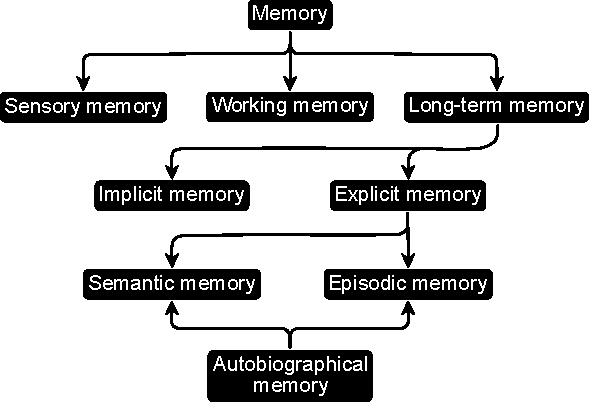
\includegraphics[width=120mm]{./Figures/Memory_overview.pdf} \caption{An overview of the different subcategories that memory can be divided into.} \label{Figure:Memory_overview} \end{figure}

Further, within long-term memory, a frequently used division is that between \emph{implicit} and \emph{explicit} memory \parencite{Reder1996}. Implicit memory here refers to the type of memory processes that are non-dependent on the person being cognizant\footnote{I am aware that the more conventional word to use here is \emph{conscious}. However, my whole master thesis \parencite{Larsson2011} was basically about arguing that this word is used in a confusing and ambiguous way, meaning that I cannot, in good faith, use it myself in this context. What I here refer to with the word \emph{cognizant} is simply that the person can report knowledge of the matter at hand.} of the process. For example, while you can be aware of the fact that you are being conditioned to associate a certain sound with getting a piece of candy, this explicit knowledge will not be the reason why you later react positively to that sound. Given this definition, implicit memory contains a plethora of memory processes such as conditioning (which the candy scenario above is an example of), priming, habituation, and motor learning.

Explicit memory, on the other hand, refers to the type of memory that \emph{do} requires cognizant processes. Here, a further division is often used, namely that between \emph{semantic memory}, \emph{episodic memory}, and \emph{autobiographical memory}. Semantic memory is the knowledge about such things as facts, concepts, ideas, and words; basically explicit memories that are decoupled from when and how they were learned. For example, to know what a quokka is\footnote{If you do not know, look it up right now!}, one does not need to know how this fact was acquired.

In contrast, episodic memory, which will be the focus of this dissertation, has been defined by \textcite{Tulving1972,Tulving2002} as the compound memory that stores the \emph{what}, \emph{where}, and \emph{when} of an event. An everyday example of this would be to remember a meeting with a group of people in terms of what happened, as well as placing all separate events into space and time. Episodic memory would here be involved in answering questions like ``Where was this person when he said this and that?'', ``What did she say?'', and ``Did this event occur before that event?". As such, testing episodic memory can involve approaching it from many different angles, using every imaginable modality. A few examples would be remembering images, routes, faces, and locations. However, the most common way to measure episodic memory is probably by asking the participants to remember words from an earlier read or heard word list. One standardized example of this is the \emph{California Verbal Learning Test} (commonly abbreviated CVLT; \citeauthor{Delis1987}, \citeyear{Delis1987}), where the subject, on multiple occasions, is asked to remember the contents of a shopping list that they continuously are given the chance to rehearse.

Finally, autobiographical memory is a form of memory about oneself \parencite{Conway2000,Conway2005}. In this regard, it encompasses specific memories of events but also more general and abstract concepts, sorted into different themes, such as knowledge about what activities one liked as a kid. As such, autobiographical memory is a form of combination of semantic and episodic memory, and will therefore not be included or further explored in this thesis.

\subsection{Mean vs. variance sex differences} \label{Mean_vs_variance}

Most, but not all, research that has been done on sex differences has first and foremost been about sex differences in means. Here, the researchers compute the average performance/behavior/characteristic for men and women separate and then compare these means. If these numbers then can be shown to be different according to some statistical method, sex differences are proclaimed.

While mean differences absolutely are useful in and of themselves, they only reveal part of the picture. For example, simply knowing that two groups differ does not automatically enable you to predict the distribution among them in the extremes, that is, among the top or bottom achievers. Here, the concept of sex differences in variance comes in handy. Basically, when investigating this concept, you compute how much variation there is \emph{within} each group and then make a comparison between them to see how much they deviate from each other. Given that you know both the mean and variance sex differences, you can now predict the ratios of the sexes in the extremes of the distribution. This is, of course, dependent on the fact that both groups are more or less normally distributed, an assumption that, in general, surprisingly often is satisfied for different types of empirical data \parencite{Frank2009}, including psychological factors.\footnote{While investigating things outside of this assumption indeed would be both interesting and probably useful, this is beyond the scope of this thesis.}

Going further, in order to keep things organized, I will first, in the very next section, focus on what has been found regarding sex differences in general, in cognition, and in episodic memory when it comes to the measured means of men and women for different traits and abilities. Then, in the section after that, I will turn to describe what has been found within these fields with regard to differences in in-group variance between men and women.

\subsection{Mean sex differences} \label{Mean_differences}

\subsubsection{General} \label{Mean_differences_General}

When it comes to sex, there are some major differences between men and women that are totally obvious, and for most individuals it is close to impossible \emph{not} to directly categorize others into either males or females. Except for the unmistakable differences such as the different reproductive system and physical appearance, there are, for example, large differences in the average strength and length between the sexes \parencite{Fryar2016}.

Turning to psychological traits, one of the most obvious differences between men and women is probably that they have dramatically different preferences for sexual and romantic partners. That is, the overwhelming majority of people are heterosexual \parencite{Bailey2016}. Further, there has been a plethora of research within psychology showing that there are sex differences for things as disperse as personality \parencite{Costa2001}, aggression \parencite{Bettencourt1996}, narcissism \parencite{Grijalva2015}, sexuality \parencite{Petersen2010}, mental health \parencite{Rosenfield2013}, economic negotiation outcomes \parencite{Mazei2015}, scholastic achievement \parencite{Voyer2014}, and pain sensitivity \parencite{Fillingim2009} just to name a few.

\subsubsection{Cognition} \label{Mean_differences_cognition}

When it comes to mean sex differences in cognition, one of the most well-researched and well-confirmed patterns is that of a difference between verbal and spatial tasks. What has been found here is that, in general, women tend to do better at tasks that are more verbal, and men tend to do better on tasks that are more spatial. In a meta-analysis by \textcite{Hyde1988}, the authors concluded that an advantage for women could be found for many verbal tasks but not for all. For example, while women excelled at verbal fluency and verbal production tasks, no differences were found when assessing vocabulary, and men even outperformed women on analogy solving. Recent, large-scale, international studies have generated similar results, where teenage girls are better than teenage boys at reading comprehension \parencite{Stoet2013} (with the advantage for females here being about three times as large as the advantage for males in mathematics, which is discussed further down) and where adult women perform better than adult men on verbal fluency tasks \parencite{Maylor2007}, a type of test where the participants are supposed to generate as many words as possible beginning on a certain letter or belonging to a certain category.

Turning to spatial/visuospatial abilities, \textcite{Voyer1995} showed in a meta-analysis that men tend to have an advantage over women here. However, just as with the verbal tasks presented above, depending on the exact type of spatial task performed, the overall pattern also differs. For example, the largest sex difference that was found in this meta-analysis was for mental rotation tasks. This difference was at its largest when the participants worked under time pressure and when the object was in 3D rather than in 2D \parencite{Voyer1995,Voyer2011}. However, men's advantage was not as strong in tasks having to do with spatial perception and dropped even more for spatial visualization \parencite{Voyer1995}. Also, mathematics might not be an ideal example of a spatial/visuospatial task, but to the extent that it is, sex differences favoring males have been found \parencite{Stoet2013}.

\subsubsection{Episodic memory}

In \citeyear{Maccoby1975}, \citeauthor{Maccoby1975} conducted a large review of sex differences for many different psychological domains, including memory where they could not find an effect. However, this might have come about because several different memory types were intermixed, and later studies have suggested that there actually are differences between men and women here. For example, in a large study \parencite{ID9011_Herlitz1997} of 1000 adults, women performed better on episodic memory tasks where they were asked to remember activities, words, facts, or objects. Even though all these tasks are not verbal \emph{per se}, they can all be supported by verbal processes. For example, even if objects are presented as images, they can be remembered as words as long as the images shown are not too abstract. In another study \parencite{ID8092_Astur1998} that investigated more spatial tasks, men outperformed women when navigating through a maze with almost no external cues. However, when the task changed so that verbal support could be used, much smaller effects were found and in some cases no sex differences at all. Further, studies investigating both more verbal and more spatial tasks in the same subjects have also been conducted, where the results have been similar to other type of cognitive tasks, meaning that women tend to perform better on more verbal oriented memory tasks while men tend to have an advantage in more spatial tasks\parencite{ID8125_Herlitz1999,ID8024_Lewin2001}. This pattern, where there seem to be a sort of verbal-spatial spectrum that goes hand in hand with the relative performance of men and women is something that has been suggested in later reviews \parencite{Herlitz2008,Andreano2009}. It should be noted, though, that men only seem to outperform women when tasks rely heavily on spatial processing, which for example is highlighted by the fact that women seem to perform better than men when it comes to object location memory \parencite{Voyer2007}.

The hypothesis that the same verbal/spatial pattern that is present for sex differences in general cognition also should be present for episodic memory would make sense; since memory is not an isolated cognitive ability, working independently of other cognitive mechanisms, one should be able to draw from skills present for non memory related processes. For example, being able to effectively structure and visualize spatial material should influence the ability to also later recall that material. As an analogy, an expert chess player should easily be able to recall complex states of the chess board in a way that a novice probably could not.

As have been presented above, circumstantial evidence already exists regarding sex differences in episodic memory and how different factors might modify it. However, no large-scale investigation of this matter --- which could confirm the verbal/spatial pattern hypothesized above as well as examine other aspects of how sex differences might vary --- has been performed. Therefore, for Study \Romannum{1} of this thesis, we conducted a large meta-analysis of this field.

\subsection{Variance sex differences} \label{Variance_differences} \subsubsection{General}

As early as \citeyear{Ellis1894}, \citeauthor{Ellis1894} suggested that men as a group varied more than women in mental and physical characteristics, and since then investigations of large data sets across regions and time have confirmed and expanded on these findings. For example, men are more variable when it comes to such things as birth weight, blood parameters, and juvenile physical performance \parencite{Lehre2009}. Further, in a recent study, not yet published, it was demonstrated that the same pattern is present for subcortical volumes, cortical surface areas, and cortical thickness and that these differences are seen throughout the lifespan \parencite{Wierenga2020}.

\subsubsection{Cognition} In 1932, a sample of 87,498 Scottish schoolchildren born in 1921 (which constituted about 95\% of all children in that cohort) had their intelligence assessed with a large test battery not designed to minimize sex differences \parencite{SCRE1933}. When \textcite{Deary2003} later analyzed the data, he could show that boys were overrepresented both in the higher and lower tails of the distribution (see Figure \ref{Figure:Deary2003}; \cite{Deary2003}), something that he concluded ``in part [might] explain such cognitive outcomes as the slight excess of men achieving first class university degrees, and the excess of males with learning difficulties.'' The same survey was repeated in 1947 \parencite{SCRE1949}, where \textcite{Johnson2008} could confirm the same pattern. However, for both surveys, boys and girls were very similar in mean intelligence. Similar patterns have been found by, for example, \textcite{Hedges1995} who investigated the performance of over 100,000 schoolchildren, tested between 1960-1992 in the United States, and found that males showed a larger variance in performance compared to females. One of the few exceptions here was associative memory (which I will come back to in section \ref{Variance_differences_Episodic_memory}). In a similar vein, \textcite{Strand2006} found that in a national sample of 320,000 UK 11-12 year-olds, boys were more variable on quantitative, and non-verbal reasoning, and that they were overrepresented in the 10\% lowest-performing students on verbal skill. This result was replicated by \textcite{Lohman2009} in the United States with an almost as big sample of school children of all ages, tested between 1984 and 2000, where the same abilities were assessed. Similarly, analyses of the \emph{Programme for International Student Assessment} (PISA) studies have shown that boys consistently are overrepresented in the top and bottom performers in mathematics compared with the sex ratios that would be expected from the mean sex differences alone, suggesting that their test score variance is larger than what it is for girls \parencite{Stoet2015}.

\begin{figure} \centering 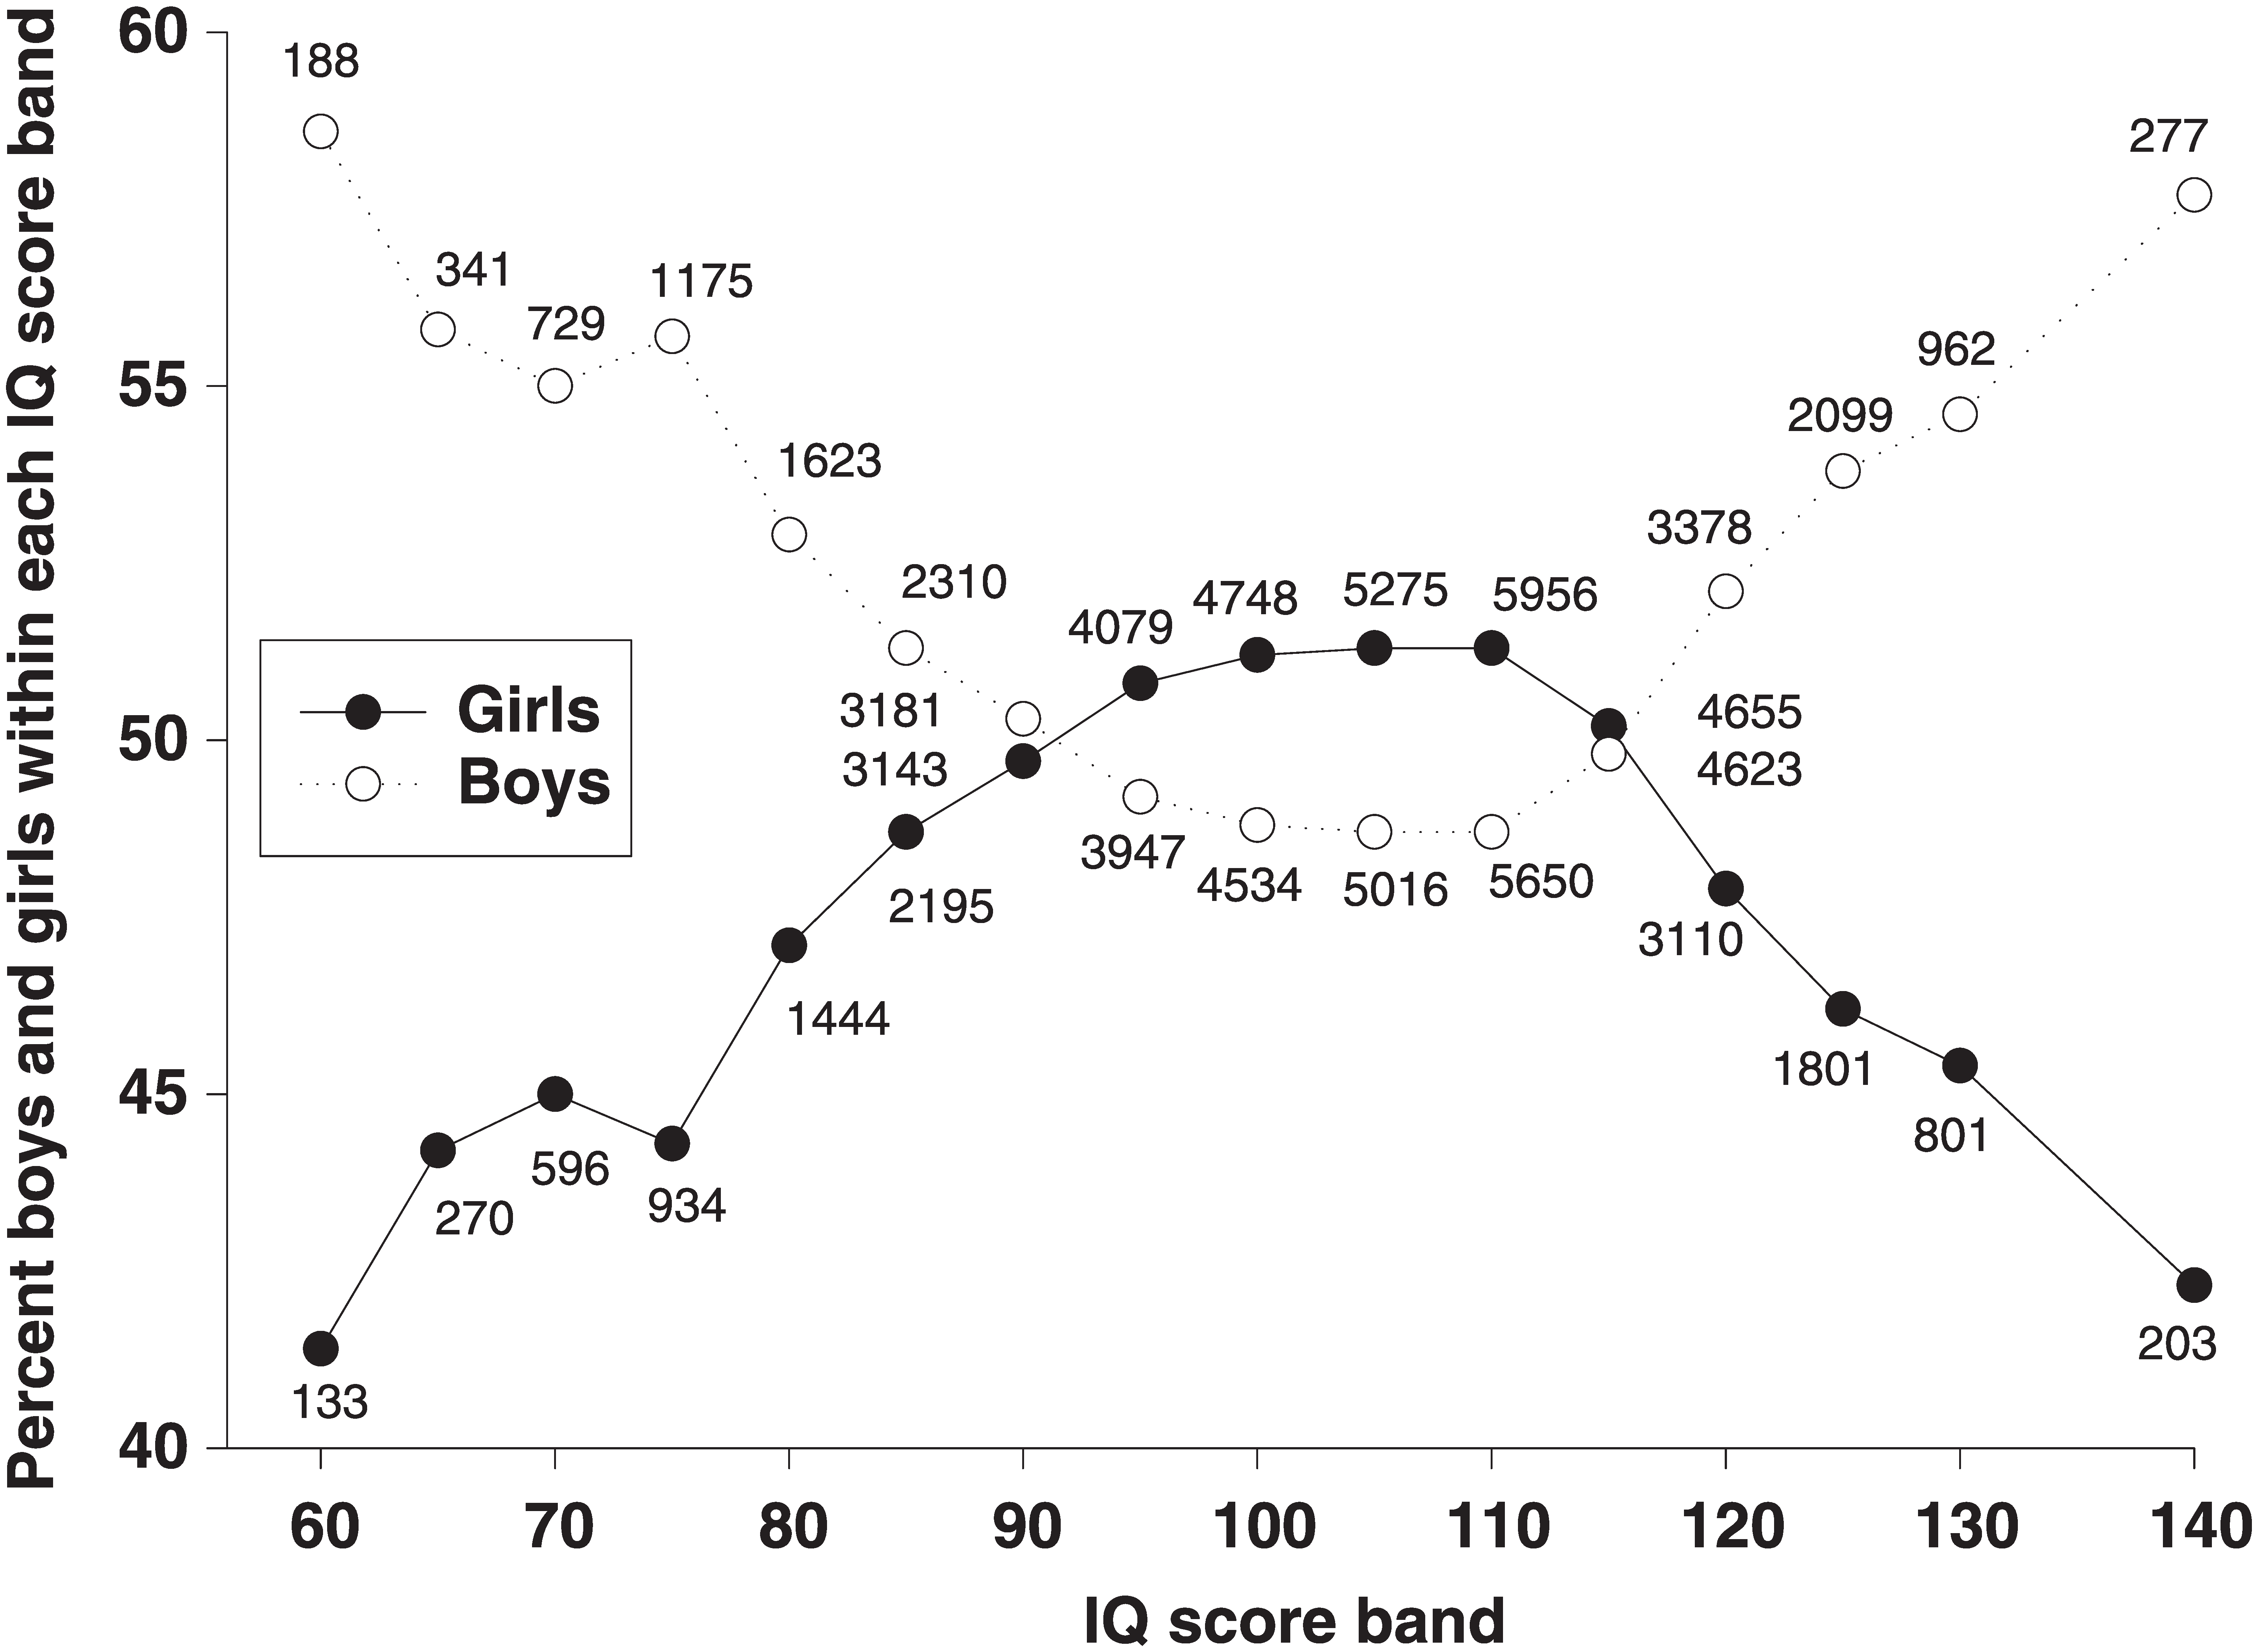
\includegraphics[width=120mm]{./Figures/Deary2003.eps} \caption{Figure 1 from \textcite{Deary2003}, showing the distribution of IQ scores in a large sample of Scottish 11-year-olds tested in 1932. Here, both the number of people as well as the total percentage of all subjects is shown separately for the two groups within 5-points wide IQ bands.} \label{Figure:Deary2003} \end{figure}

However, this pattern of larger variances in the male group is not always found. In addition to associative memory, \textcite{Hedges1995} found no consistent variance sex differences in reading comprehension and perceptual speed. Further, when \textcite{Irwing2005} conducted a meta-analysis of 22 studies from around the world on progressive matrices performance (a task where you have to guess the last part of a given pattern of abstract forms) in university students, they found that while men had a higher performance average, women were more variable on the standard version of the test compared to the more advanced where no variance differences were found. Also, in a large, population-based Romain sample, no variance sex differences could be found either for general intelligence or for more specific, second-level cognitive abilities \parencite{Iliescu2016}.

\subsubsection{Episodic memory} \label{Variance_differences_Episodic_memory}

To my knowledge, there has been no other investigation of sex differences in variance for episodic memory except for the study by \textcite{Hedges1995} mentioned in the previous section, where associative memory in three national U.S. surveys --- in total comprising over 100,000 school children ---  was investigated. Here, results showed no clear pattern, with one sample showing larger variance for boys, one showing larger variance for girls, and one showing neither. Since the result of this investigation in variance differences in itself was highly variable, and since only one specific type of memory task was investigated, this means that more research is needed in order to say something regarding this matter. This will be the focus of Study \Romannum{2} of this thesis.

\subsection{Explanations of sex differences}

So far, I have mostly described what sex differences there are without really touching on any explanations for \emph{why} these sex differences also exist, a question I will now turn to. Here, it is important to bear in mind that what constitutes an explanation depends on what perspective you are interested in. For example, you could propose why something should be the case by referring to how adaptive it has been during the course of evolution. However, this does not mean that you now understand \emph{how} it comes about any more than understanding \emph{why} humans build bridges helps you understand \emph{how} bridges are built. Similarly, you could put forth an explanation that a cognitive function activates a certain part of the brain more than another, but without a grander perspective of the ins and outs of how the brain works and give rise to human behavior this has limited explanatory power (see \citeauthor{Eric2017}, \citeyear{Eric2017}).

Given the reasoning above, the best way to understand why sex differences might arise is to approach the question from several different point of views. For the scope of this thesis, I will try to make a contribution regarding one of these perspectives, namely a societal explanation. However, I will start by going through both possibly evolutionary and biological explanations.

\subsubsection{Evolutionary explanations} \label{Evolutionary_explanations} I will call something an \emph{evolutionary explanation} if the way things are can to some extent be derived back to what has been beneficial for the spreading of certain genes that controls the phenotypic expression in question. From a theoretical point of view, major sex differences should only appear in a species if males and females have different roads to achieve reproductive success (which, evolutionarily speaking, is the only thing that matters), something that in turn only can be the case if the sexes' differ in what roles they play in the reproductive process (which they do since this is what defines sex in the first place). A clear example of this would be something that already has been touched upon in section \ref{Mean_differences_General}, namely that most people are heterosexual \parencite{Bailey2016}, which in turn means that men and women are attracted to dramatically different attributes in other humans. This can simply be derived back to the fact that historically, those individuals that were more attracted to the same sex did not procreate to the same extent as those that were more attracted to the opposite sex, in turn leading to genes controlling for homosexuality being less prevalent in the gene pool. However, this explanation breaks down at a certain point, and there are a number of theories regarding why, in an overwhelmingly heterosexual environment, it might be evolutionarily beneficial to be or lean towards homo- or bisexuality \parencite{Savolainen2016}. For example, one such theory suggests that male homosexuality can be beneficial for an individual with an older brother, since it decreases competition for resources necessary for mating, thereby giving the sibling a sort of \emph{carte blanche} to finding one or several suitable mates, something that will benefit the homosexual individual as well since he shares, on average, half his genes with his brother, which in turn will be passed on to the brother's children \parencite{Apostolou2013}.

Moving one, one of the most important differences between males and females when it comes to the reproductive process is that males, in theory, can have an almost infinite number of offspring while females are restricted by the number of pregnancies\footnote{In order to not have this section being longer than the rest of the thesis combined, I am going to restrict myself to only speak about mammals. So no egg-laying, sequential hermaphroditic, male pregnancy activities allowed!} they can fit during their lifetime.\footnote{As a concrete example, it has been suggested that about 0.5\% of all males in the world are ancestors to Genghis Khan, the emperor of the Mongol Empire who lived less than a thousand years ago \parencite{Zerjal2003}, something which probably was achieved by him having several orders of magnitude more children than what a single woman ever could have.} Further, a consequence of this is that in order for a male to spread his genes through means of having a child, the theoretically lowest amount of resources that he would have to devote would be the time and energy it takes to have sex with a female. He could then move on, and if the female does not make it on her own, his losses would, evolutionary speaking, be minimal given his investment. On the other extreme, he could plow all his resources into the female during pregnancy and the child postnatally. While both of these pathways could be successful strategies, their feasibility would depend on the male's other traits and qualities, as well as the environment in which he operates. That is, the strategy of impregnating a lot of females would probably not be especially effective for an unattractive male who will be given limited opportunities for coitus. Neither would it be a good strategy if there were a real shortage of other females to impregnate. On the other hand, in order for a female to have a child, she will \emph{at minimum} have to go through a long, very resource-demanding pregnancy (and in the case of humans, historically a rather high risk that either she, her offspring, or both perish during childbirth), during which she will not be able to reproduce with someone else. This immediately narrows her options for successful strategies compared to a male. For example, abandoning the child would be a sort of evolutionary chicken race where the mother almost always would have more to lose from it than the father. Also, having sex with any random, willing male would for a time block her from later having children with a more suitable male. The point here is that from an evolutionary perspective, males have a large spectrum of strategies to draw from when it comes to successfully spreading their genes through means of procreation.

When it comes to variance sex differences, as already have been covered in section \ref{Variance_differences}, males tend to be more variable than females. One theory that has been put forth to explain this pattern links it to the different strategies for procreation outlined above \parencite{Moore1991}. According to the theory, because of the larger set of viable strategies available for males compared to females, there would also be a larger set of different phenotypes present in the male group compared to the female group. This would, in turn, translate into larger variance for different traits and skills for males as a group. \footnote{\label{Footnote:Frontiers} A brief version of this explanation had to be removed from Study \Romannum{2} in order for the paper to be accepted because it was judged by the journal to potentially drive a sexual stereotype.}

Depending on different circumstances, species can evolve toward being more or less monogamous/polygamous \parencite{Kleiman1977}. For example, if partners are scarce, it might pay off for males to stay and guard their mate against other suitors rather than to look for new mates \parencite{Schacht2016}. Here, it has been shown that monogamous species exhibit less sex differences than polygamous species because their roles will more overlap in the former scenario \parencite{Gaulin1992}. For example, while it may pay off for a polygamous male to have a large body size --- something that ultimately might let him compete with other males and impregnate a lot of females --- if he is monogamous, the cost of having a large body size makes less sense since the potential payoff is smaller.

The same pattern described in section \ref{Mean_differences_cognition}, that men generally perform better on spatial tasks than women, has also been seen in many animals such as mice, rats, voles and monkeys \parencite{Jacobs1990, Gaulin1992, Jones2003}. There are a number of different evolutionary theories regarding why males are better at spatial tasks where the one with the strongest support relates it to range size. More specifically, males in polygamous species usually have larger territories than the females whereas these two tend to overlap in monogamous species. This is a consequence of the polygamous males having a strategy to find and mate with many different females as opposed to just one as is the case with the monogamous males. Here, it has been seen that in species where males have larger range size than females, they also perform better than the females on spatial tasks, something that is not seen in species where the sexes have more equal territorial sizes. It is hypothesized that the underlying reason for this relationship is that males with larger range sizes than females also need better spatial skills, since navigating around in the environment is something that they need to be more proficient at. Since humans are not strictly monogamous creatures, this could then, at least partly, explain why men perform better than women on spatial tasks. One could, in a similar way as above, speculate about how women might be more benefited by verbal skills than men. However, since only humans display verbal skills, there are no animal studies regarding this matter. An evolutionary explanations would therefore be more of a just-so story, something that can be useful but still has less scientific proof than explanations like the ones for sex differences in spatial cognition presented above \parencite{Holcomb1996}.

\subsubsection{Biological explanations} \label{Biological_explanations}

I will call something a \emph{biological explanation} if the state of things can be related to the constitution of some biological traits, such as the composition of the genes or the structure of the brain. On the genetic level, what differs between men and women is that for the 23\textsuperscript{rd} chromosome pair (the so-called sex chromosomes) women have an X chromosome while men have a Y chromosome, meaning that men in total have fewer base pairs of genetic code than women. Even though these genetic differences alone should give rise to some phenotypic disparaties between men and women, most sex differences probably comes about because of gene/hormone interactions \parencite{Gaulin1992}, meaning that autosomal genes (that is, genes not located on any of the sex chromosomes) are expressed differently depending on the hormone environment, which in turn often is a stable indicator of the sex of the individual. It is unclear exactly to what extent psychological sex differences arises because of this mechanism, but some evidence points to, for example, spatial abilities being affected by it \parencite{Berenbaum2016}.

Focusing on the genetic differences alone (that is, without the influence of hormones), one theory \parencite{Reinhold2013} has tied this to the fact that men seem to be more variable than women (see section \ref{Variance_differences}). That is, for the overwhelming majority of all genes, their phenotypic expressions are influenced by two versions of the gene, one on each chromosome. This means, for example, that mutations of one copy of the gene in many cases can be counteracted by the other copy. However, for men, when it comes to genes on the sex chromosomes, some of these only have a single version since there are some genes ``missing'' on the Y chromosome. This has the effect that mutations on these base pairs more often actually are expressed for men, which in turn means that they show a larger variance than women. In addition, it should be said that for some species, females have the XY chromosome pair, meaning that \emph{they} should be more variable instead, something that, for example, has been shown when it comes to body size \parencite{Reinhold2013}.

Turning to the brain itself, if there are differences on the group level between men and women when it comes to behavior and cognitive performance, as have been shown in section \ref{Mean_differences} and \ref{Variance_differences}, these differences \emph{have} to be manifested in the nervous system somehow. \footnote{This logic holds even for mind-body interaction dualist like myself as long as the belief is held that the mind to at least some extent relies on the brain to carry out behavior and perform computations, a position that just about every scientist and philosopher probably would agree with.} However, one could pose the question of to what extent the brain differences that have been detected also are linked to behavioral and performance differences, and if so in what way \parencite{Grabowska2016,McCarthy2016}. That is, even if observed discrepancies in behavior and performance \emph{have} to have brain-based explanations, it is still possible that other brain differences than the ones that already have been found are responsible.

When it comes to biological differences in the brain, it has been confirmed that there are differences in neuroanatomy, neurochemistry, physiology, and connectivity \parencite{Andreano2009,Tian2011,Ingalhalikar2014}. Men and women also tend to differ in many cases with respect to how the brain processes information. For example, sex differences have been found in how men and women process faces \parencite{Proverbio2017}, as well as emotional expressions in others \parencite{Kret2012}.

Further, observable brain differences do not automatically have to lead to observable behavioral differences, one possible reason being that the behavioral consequences simply are too small to detect. However, the same type of behaviors could also be manifested through different brain processes. \textcite{Haier2005} have for example shown that IQ is correlated with activities in different areas of the brain for men and women. While the frontal lobe is important for both sexes, men seem to rely more on the parietal lobe and women on Broca's area. Further, \textcite{Jordan2002} showed that men and women who are equally good at mental rotation tasks nonetheless showed differences in brain processing. The take-home message here is that when studying the brain, one has to be careful drawing conclusions about behavior.

Differences in the brain between men and women have also been found when it comes to episodic memory. For example, \textcite{Young2013} found several brain discrepancies between the sexes for autobiographical memory irrespective of the valence of the content, something that they interpreted to reflect sex-specific cognitive recall strategies. Further, on a test of two different episodic memory tasks --- more specifically \emph{Wechsler Memory Scale - Revised} (commonly abbreviated WMS-R) and the California Verbal Learning Test (already described in section \ref{Definition_of_episodic_memory}) --- \textcite{Ragland2000} found that performance for women, but not men, was correlated to activity in the temporal pole.

\subsubsection{Social explanations} \label{Societal_explanation}

I will call something a \emph{social explanation} if it comes about because of the social environment that a person grows up and/or live in.\footnote{However, it is important to note that explanations like these never can be fully decoupled from evolutionary explanations, the likes I went through in section \ref{Evolutionary_explanations}. In the words of \textcite{Gaulin1992}: ``Any claim that `x is the result of experience' must explain why experience has that particular effect rather than any of an infinite array of possible effects. Such explanations can only be evolutionary.''} As such, there are many different type of potential social explanations that could be brought up when it comes to sex differences, for example, how the behavior of families, friends, and strangers might affect the sexes differently, or how stereotypes and gender roles might have an influence. However, for this thesis, I will focus on grander, more societal explanations, and this is also what we will investigate further in Study \Romannum{3}.

The \emph{Flynn effect}, first described by James Flynn in \citeyear{Flynn1987}, is a term that describes the phenomena that has been observed for over 100 years where the IQ scores steadily have gone up over time all across the globe \parencite{Williams2013}. Some factors that have been suggested as explanations for this effect are increased education, gradually smaller family sizes, and improved health care \parencite{Pietschnig2015}. This is supported by the fact that the Flynn effect is largest in parts of the world that have experienced the most dramatic increase in living conditions (see for example \citeauthor{Weber2017}, \citeyear{Weber2017}).

Some researchers have proposed that there is a link between improvements in living conditions, like the ones mentioned above, and increases in women’s cognitive performance when compared to men's, in a way suggesting that the Flynn effect and similar phenomena are affecting the sexes differently. One explanation for why this might be the case could be that in underdeveloped regions, women tend to have less access to social goods, for example education, than men. Possibly then, when living conditions increase in general, women may benefit more. That is, imagine a purely illustrative example where the average boy in a certain country goes from spending five years in school to ten while the average girl goes from getting no education at all to spending five years in school. Even though both sexes are given five extra years in school, it stands to reason that girls should experience a larger improvement than boys in for example mathematical ability (even if boys still perform better in absolute terms) because of diminishing returns that might affect boys to a larger degree.

As a concrete example of this pattern, \textcite{Guiso2008} investigated the 2003 cross-cultural and cross-sectional PISA survey of mathematic competence in 15-year-olds found that while boys generally perform at a higher level then girls, in countries with relatively high gender equality, this advantage for boys was smaller. Conversely, in these countries, the advantage for girls in reading comprehension was further enlarged. Finally, it could also be seen that the difference between mathematical ability and reading ability shrunk for girls when gender equality increased, something that was not the case for boys. \textcite{ElseQuest2010} extended these findings by investigating the 2003 PISA data together with data of 15-year olds from the 2003 cohort of the \emph{Trends in International Mathematics and Science Study} (TIMSS). Again, results showed that females' relative mathematical performance in comparison to males was positively associated with increases in gender equality. Further, \textcite{Weber2014} carried out an investigation of the \emph{Survey of Health, Aging and Retirement in Europe} (SHARE) data, in which the subjects are older than 50 years and live in Europe. Here, yet again, results showed that improved living conditions and more gender-inclusive education were related to relative improvements in women's performance in comparison to men for verbal episodic memory (which I will come back to shortly), numeracy, and category fluency.

However, \textcite{Stoet2013,Stoet2015} have questioned the generalizability of some of these results, claiming that the PISA data only show these patterns for the 2003 cohort, while the cohorts from 2000, 2006, and 2009 lacked this relationship. Further, \textcite{Lippa2010c} studied line angle judgment and mental rotation performance in 18-40 year-olds from 53 different countries tested online and found that men not only performed better than women in all counties tested, but also that these sex differences were greater in men's favor in countries with more gender equality, something that runs contrary to the pattern suggested above.

Turning to episodic memory, the overall pattern has been more consistent. Here, two large scale investigations have been performed. First, as already mentioned above, when \textcite{Weber2014} investigated data from the SHARE study, they concluded that when comparing with men, women's relative performance on episodic memory increased with better living conditions. Second, \textcite{Bonsang2017} investigated how sex differences in verbal episodic memory performance were moderated by gender equality values in society across both regions and age groups. More specifically, performance data on episodic memory from the \emph{U.S. Health and Retirement Study}, the \emph{Survey of Health, Ageing and Retirement in Europe}, the \emph{English Longitudinal Study of Ageing}, and the \emph{World Health Organization Study on Global AGEing and Adult Health} was used in conjunction with participant judgments from the \emph{World Values Surveys} regarding if they agreed with the statement ``when jobs are scarce, men should have more right to a job than women'' as well as the number of protestants in each country (which was interpreted as a proxy of conservatism on gender issues). Results showed that both of these measures were linked to women's relative improvement in verbal episodic memory compared to men's (see Figure \ref{Figure:Bonsang2017}).

\begin{figure} \centering 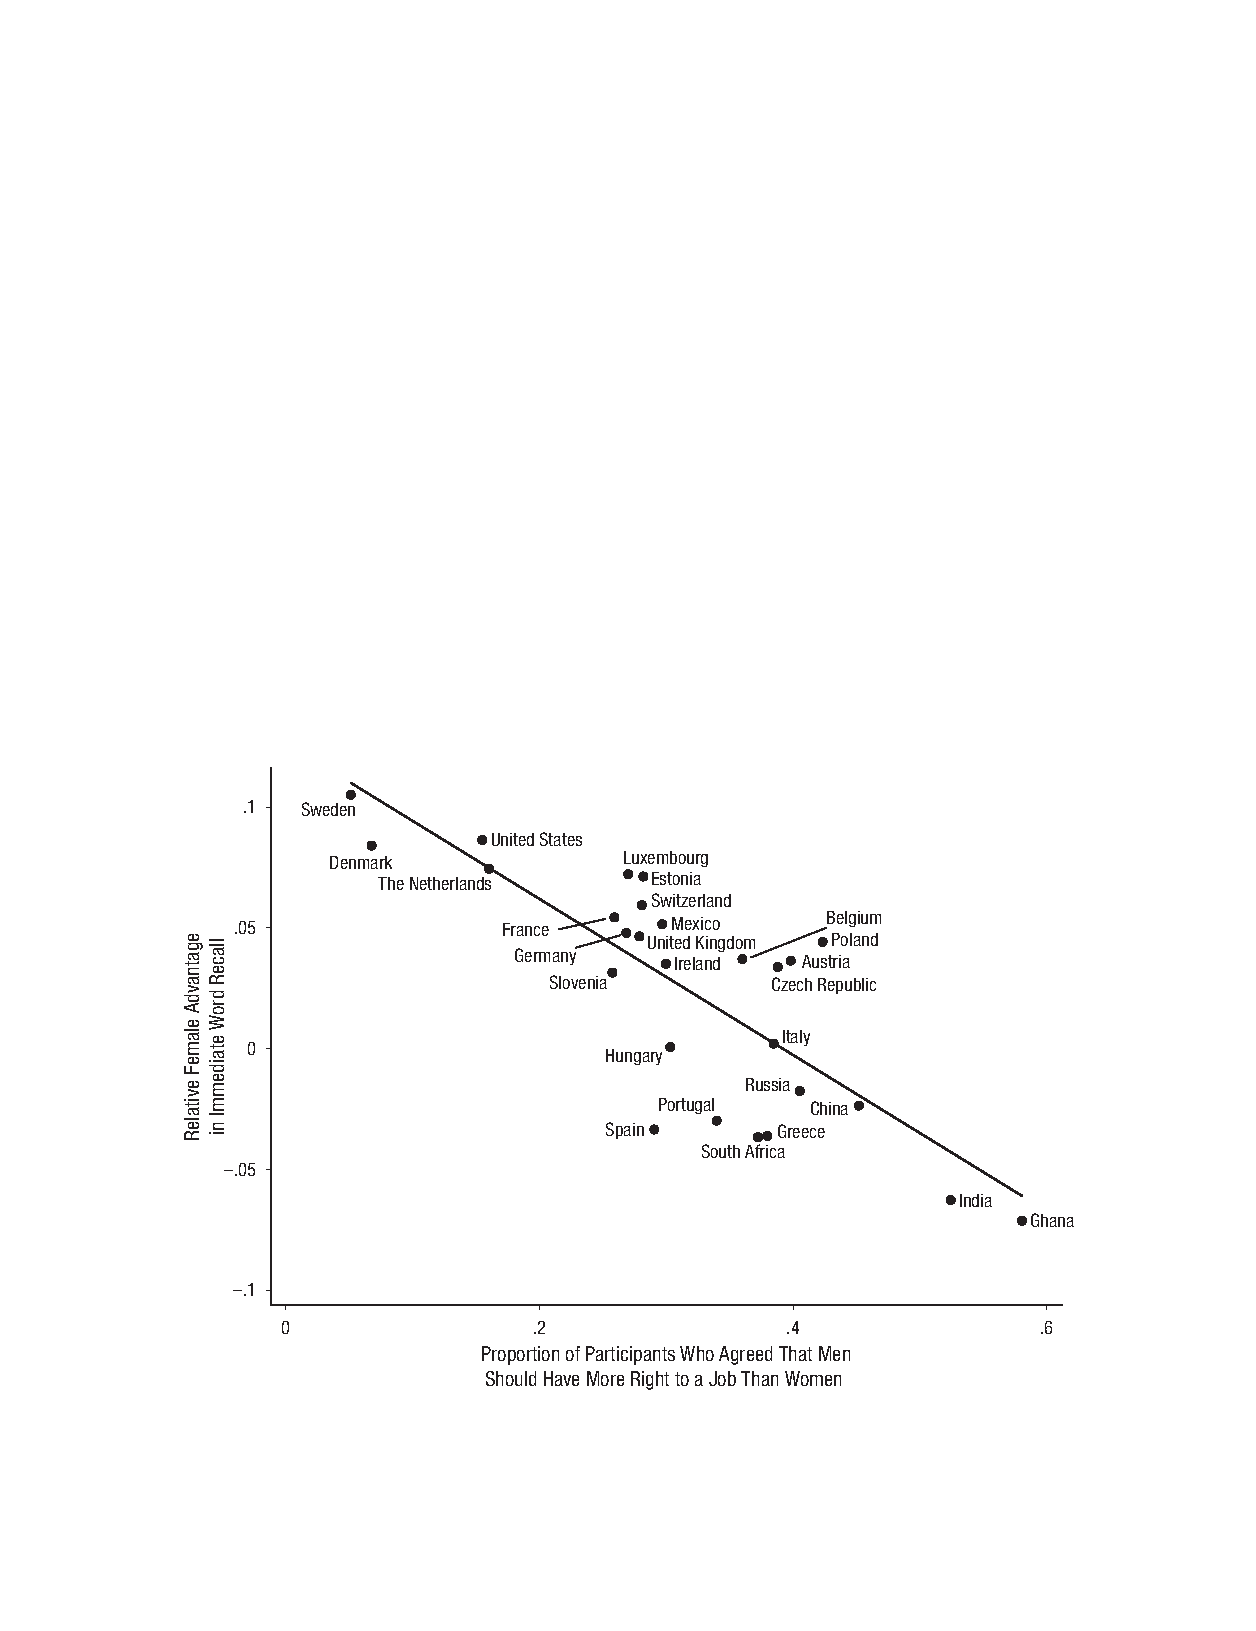
\includegraphics[width=120mm]{./Figures/Bonsang2017.pdf} \caption{Figure 1 from \textcite{Bonsang2017} showing, for each country, the association between relative female advantage (compared to men) in word recall and the proportion of people over 50 years in age agreeing with the statement: ``When jobs are scarce, men should have more right to a job than women''.} \label{Figure:Bonsang2017} \end{figure}

Importantly, both studies presented above \parencite{Weber2014,Bonsang2017} were performed on datasets where participants were above 50 years of age. While the data collections were not spread out in time, the authors of both studies used different values for the predictor variables for each age group in each country. For example, when \textcite{Weber2014} investigated GDP per capita for a certain age group from a certain country, they used the GDP per capita value from the year when the participants in that age group were about 25 years old. This was then combined with other measures, handled similarly, to derive a regional development index for each specific age group in each specific country. One way that the results from these studies could be expanded upon would be to incorporate data from even more countries, collected at many different time points instead of a very narrow time frame. This is what will be done in Study \Romannum{3} of this thesis.

\subsection{Overarching research questions} \label{Research_questions}

For this thesis, there are three overarching research questions/themes that will be investigated through three different studies:

\begin{enumerate} \item Do men and women differ at the group level when it comes to mean differences in episodic memory performance and, if so, what factors influence this difference? This will be investigated in Study \Romannum{1}. \item Do men and women differ at the group level when it comes to variance differences in episodic memory performance and, if so, what factors influence this difference? This will be investigated in Study \Romannum{2}. \item Are men and women affected differently by societal progression when it comes to mean differences in episodic memory performance? This will be investigated in Study \Romannum{3}. \end{enumerate}

\section{Method} \subsection{Dataset} \label{Dataset}

In order to investigate the research questions outlined in section \ref{Research_questions}, we set out to create a dataset of relevant studies. More specifically, our goal was to capture as much as possible of the research that had been conducted on episodic memory where both men and women were tested.

\subsubsection{Data collection} \label{Data_collection}

Two different database queries were performed (see Figure \ref{Figure:Flow_chart} for an overview of the whole data collection phase). The first one was performed in \emph{PsycINFO} and \emph{Medline} and spanned from January 1972 to September 2001 where the search terms ``memory'' and ``sex OR gender'' were used. The term \emph{episodic memory} has not been used consistently in the literature, which is why the broader concept \emph{memory} was used instead. Also, not adding the ``sex OR gender'' would surely result in more relevant studies showing up, but this search resulted in over 65,000 abstracts, which was practically infeasible to go through. Instead, the final search resulted in 2,425 abstracts.

\begin{figure} \centering 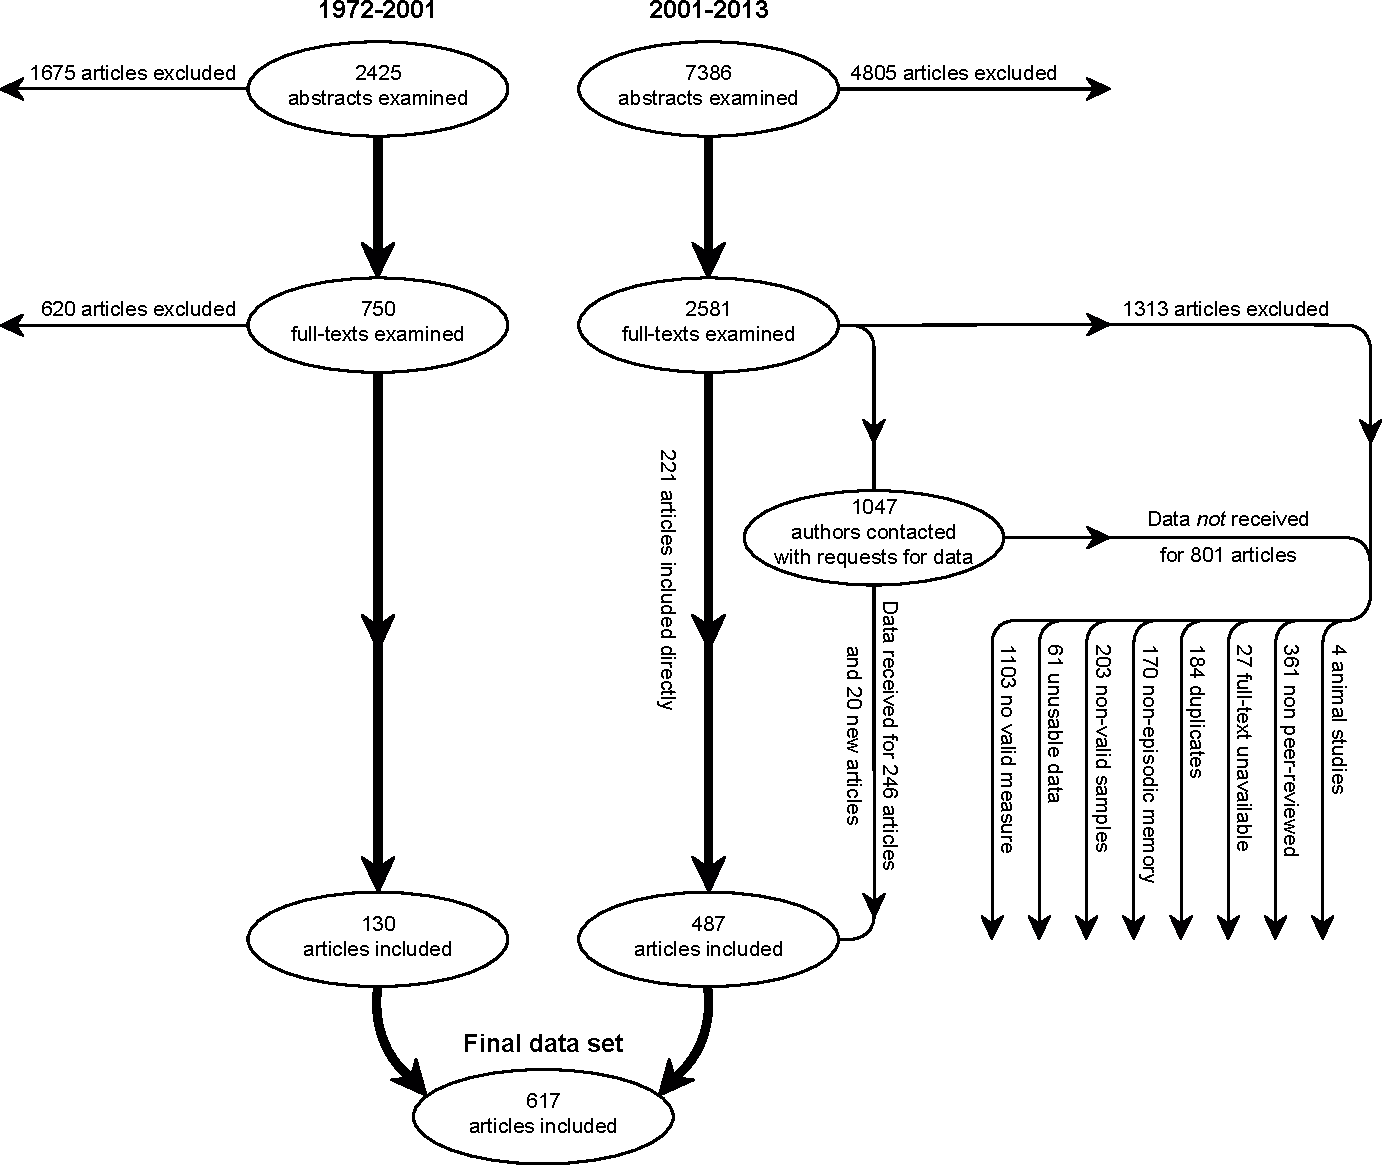
\includegraphics[width=120mm]{./Figures/Flow_chart.pdf} \caption{Figure 1 from \textcite{Asperholm2019} depicting the data collection phase of the dataset that constituted the basis of the studies in this thesis.} \label{Figure:Flow_chart} \end{figure}

The original intention was that Study \Romannum{1} would be completed after this first search, a plan that never was realized. Instead, when enough time had passed since the first search, an additional database query had to be performed to get the dataset up to date. This database search was performed in \emph{PubMed} and \emph{PsycINFO}, spanning from September 2001 to 25 November 2013. Here, the search terms ``memory'', ``sex OR gender'', and ``humans'' were used, the last term added to even further narrow the results. This resulted in 7,386 abstracts.

After retrieving all abstracts, the next step was to go through them and, if deemed interesting, retrieve the full text to investigate them further. For the first search, full-text articles were retrieved if it somehow was indicated in the abstract that males and females had been compared or if this could be reasonably suspected. For the second search, this process was even more inclusive where full-text articles were retrieved if it could not be ruled out from reading the abstract that both males and females had performed some kind of episodic memory task.

There were four main criteria that each study/sample/measure needed to satisfy in order to be included in the final dataset:

\begin{enumerate} \item The study had to be published in a scientific, peer-reviewed journal (meaning for example that book chapters and dissertations were not included), and the data had to be unique for that particular study (meaning that if several articles used the same dataset, we kept the one deriving the outcome on the largest amount of participants). \item The participants that partook could not have been selected based on some type of illness, disease or disorder, and they could not have been subjugated to any type of experimental manipulation that seriously may have affected their memory performance. This meant that while, for example, different type of health conditions could be represented in the dataset, its prevalence in the sample should more or less reflect the prevalence of that condition in the general population. \item All participants had to be exposed to the same material during the encoding phase. For example, questions of what you ate for breakfast would not qualify since different participants would have eaten different meals (or maybe even nothing), meaning that the difficulty of the task would vary between them (not to mention that it is impossibe for the experimenter to know the correct answers). \item A direct measure of episodic memory accuracy, such as the number of words remembered from a previously seen word list, had to be reported. This means that, for example, total response time would not qualify since this would measure how fast, rather than how accurate, someone remembered something. \end{enumerate}

All articles that had been selected for inclusion in the first data collection phase were reexamined and recoded in the second data collection phase in order to achieve a high level of consistency between the two searches.

In many cases, the researchers had no intentions of investigating differences between the sexes but rather to examine episodic memory with regard to some other aspect. Therefore, for the second data collection phase, if it was suspected that episodic memory performance data for both males and females existed, and if the article was not published more than ten years prior, a couple of requests to get the relevant data was sent out to the authors via e-mail. In total, 1047 authors were contacted, which resulted in us receiving unpublished data for 246 articles that we could use. In addition, we could sometimes be redirected to other articles where the relevant data had been published. Finally, sometimes the dataset used in a certain article came from a large, open database. Whenever this was the case, we went to the original source, something that resulted in four large databases being included in the study. These databases were: \emph{Survey of Health, Ageing and Retirement in Europe} (SHARE; \citeauthor{Borsch2013}, \citeyear{Borsch2013}), \emph{The English Longitudinal Study of Ageing} (ELSA; \citeauthor{Steptoe2012}, \citeyear{Steptoe2012}), \emph{Health and Retirement Study} (HRS; \citeauthor{Sonnega2014}, \citeyear{Sonnega2014}), and \emph{Study of Global Ageing and Adult Health} (SAGE; \citeauthor{Kowal2012}, \citeyear{Kowal2012}).

All in all, 617 studies were included in the final dataset, constituting 4,171 individual effect sizes, 1,370 independent samples, and 1,233,921 participants (with 564,433 males and 669,488 females). The full or a partial set was then used for all studies that we conducted in the context of this thesis.

\subsubsection{Hierarchical structure of the data} \label{Hierarchical_structure}

The final dataset had a certain hierarchical structure to it: Every study could be made up of several different samples. For each of these samples (for example young and old participants), participants could have performed several different tasks (for example remembering words and remembering images), and for each of these tasks, several different outcomes could be measured (for example free and cued recall). This means that a study could consist of just one effect size (if just one measure was taken from one task for one sample) or many. For a visual illustration of this structure, see Figure \ref{Figure:Study1_Explanation}, and for a discussion on how this structure needs to be handled statistically, see section \ref{Dependency} (the upshot of that discussion being that the standard meta-analytic procedure should not be used, but rather a model specifically tailored to deal with dependency structures like these).

\begin{figure} \centering 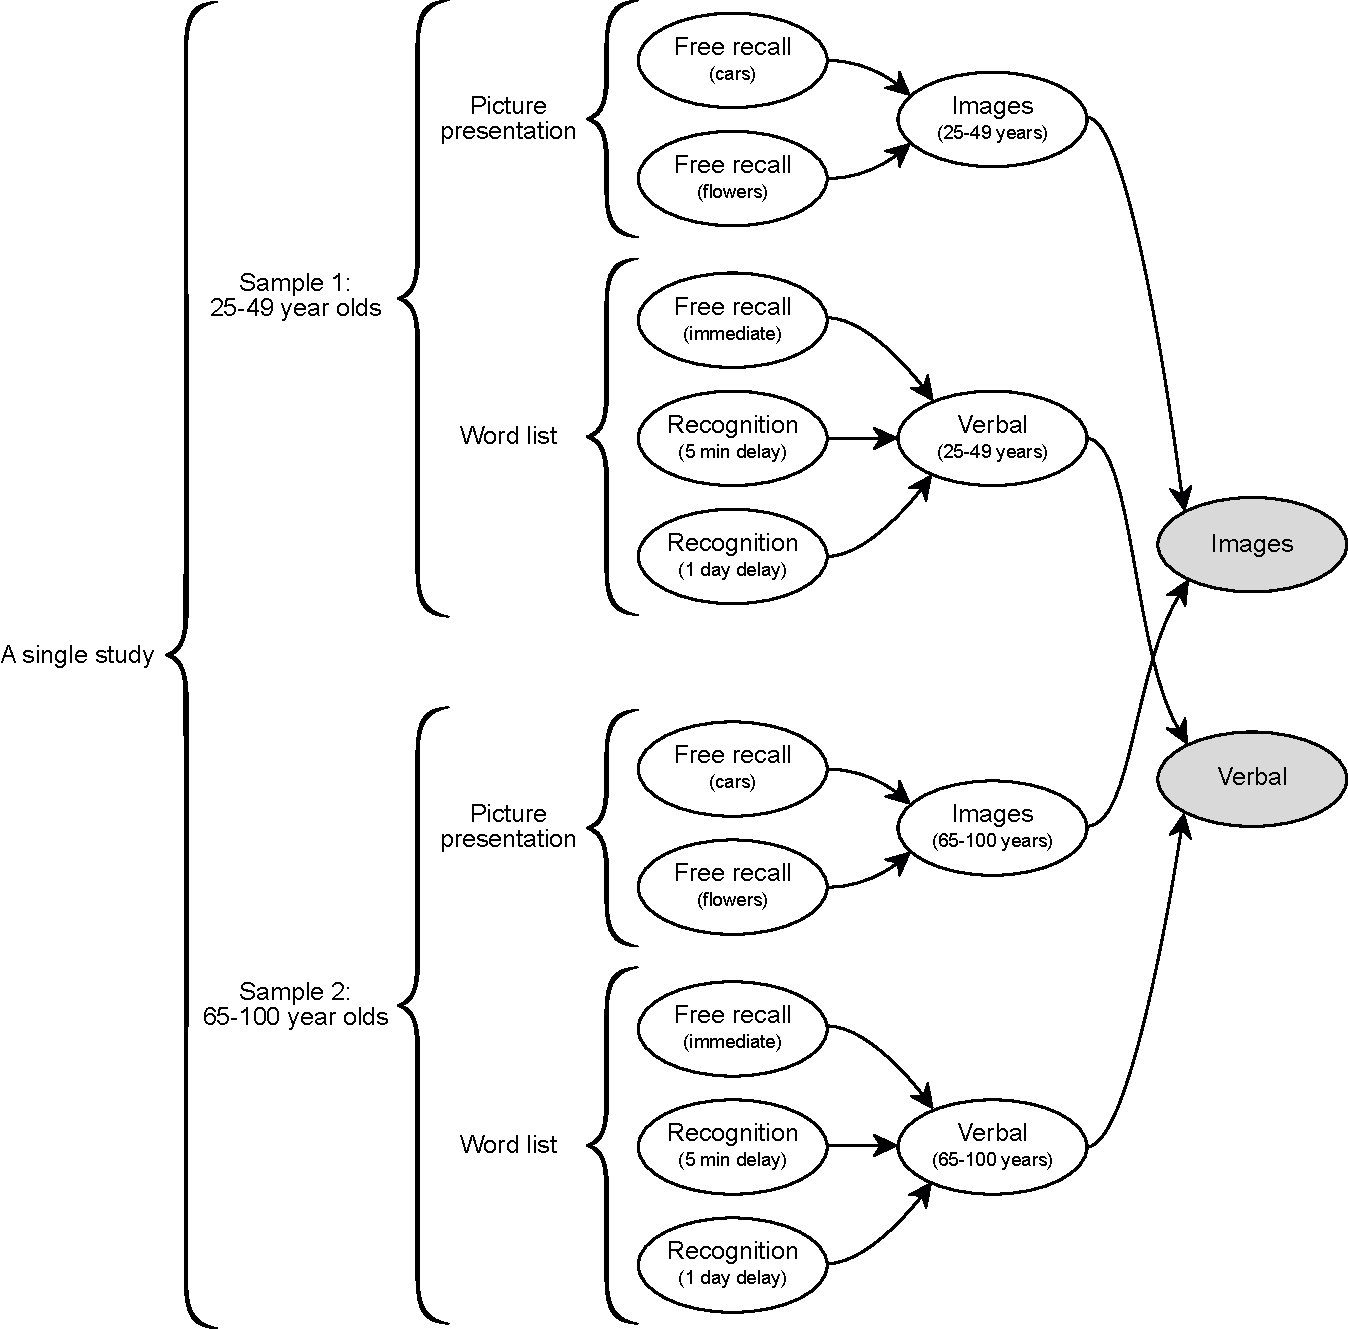
\includegraphics[width=120mm]{./Figures/Study1_Explanation.pdf} \caption{Figure S1 from Study \Romannum{1} depicting the hierarchical structure of the data described in section \ref{Hierarchical_structure}. Here, a specific example is shown where two samples have been tested on two different tasks with several outcomes each. It is then showed how these different data points contribute toward a certain moderator, more specifically different levels of what type of material that was supposed to be remembered (see section \ref{Moderators}).} \label{Figure:Study1_Explanation} \end{figure}

\subsubsection{Moderators} \label{Moderators} In addition to the data needed to compute an effect size (see section \ref{Effect_sizes}), a lot of other variables were recorded for each data point that then functioned as the basis for several different moderator analyses and subset divisions in the different studies. Most of these variables were only analyzed in Study \Romannum{1}, but some of them were used throughout all of the studies. The most used variable, that in one way or the other was used in all three studies, was \emph{type of material} to be remembered. This division consisted of eight separate levels, ranging from highly verbal to highly spatial, although for three of the levels (\emph{faces}, \emph{sensory}, \emph{remaining}) this scale was not applicable. More specifically, these categories were:

\begin{description} \item [Verbal.] Words, sentences, facts, and conversations. \item [Images.] Images of real or abstract objects and scenes. \item [Movies.] Movie clips with or without sound. \item [Locations.] Locations of objects. These tasks usually took the form of either having the participants placing objects where they previously had been or having them indicate what object previously had been at a certain spot. \item [Routes.] Routes through space. These tasks could, for example, be about memorizing a path on a map or remembering the way through a 3D maze. \item [Faces.] Images of human faces. \item [Sensory.] Odors, tastes, and colors. \item [Remaining.] Material that could not be placed within one of the above categories, such as composite measures based on several of them, or simply tests that were not described in enough detail to make a confident judgment about which category to place them in. \end{description}

Another set of variables that were used both in Study \Romannum{1} and Study \Romannum{2} pertained to possible bias in the dataset. More specifically, the following four variables were defined:

\begin{description} \item [Database search.] The distinction brought up in section \ref{Data_collection} between studies gathered in the 1972--2001 or 2001--2013 database query. \item [Data source.] The distinction brought up in section \ref{Data_collection} between data that were recorded directly from published articles and unpublished data that were retrieved from authors via e-mail. \item [Study objective.] The distinction between whether the goal of the study was to investigate sex differences or not (which was most often the case). \item [Sampling of subjects.] The distinction between whether the sample used for a particular study was convenience based (which most often was the case) or if it was population-based, meaning that the authors made a serious effort to have the sample accurately represent the population they were investigating. \end{description}

Finally, yet two more continuous variables that were used both in Study \Romannum{1} and  Study \Romannum{2} were defined the following way:

\begin{description} \item [Age.] A continuous value representing the sample age. Whenever a mean age was given, this was also used as the \emph{age} value of the sample. However, sometimes only an age range was given. In this case, the middle value of that age range was used as the \emph{age} value of the sample. \item [Year.] The publication year of the study from which the data point was taken. \end{description}

\subsection{Statistics} \label{Statistics}

\subsubsection{Basics of meta-analyses} \label{Basic_meta-analyses} For all studies included in this dissertation, the meta-analytic method was used for the main analyses, although it is important to note that this does not automatically make the studies into traditional meta-analyses. Rather, as will be seen, the meta-analytic method can --- or even \emph{should} --- be applied to any type of data where the individual data points have some known variance, preferably with some kind of measure that can be used to weight the different data points according to how precise these variances can be assumed to be (in our case, that would be the number of participants in a sample). This can be contrasted to most common statistical analyses such as a simple t-test or an ANOVA, where the dependent variable usually only is a set of numbers that represent individual measuring points (meaning that they have no inherent variance).

So, when you have aggregate data as your raw data, meaning that you have both the mean and the variance for each data point, you can use this variance to weight each data point in the final estimate. Even better, if you know how many individual measuring data points each aggregate data point is made up of (in our case, the number of participants), you can compute a weighted variance based on how precise the data point in question can be assumed to be. That is, if you in your dataset, consisting of aggregated variables, would disregard the weighted variance of individual data points, you would also end up not knowing whether one aggregate data point comes from sampling something 10 or 10,000 times, information that you would like to have in order to weight them properly. So, for example, if you had aggregated data from a study with 10 participants and from a study with 10,000 participants where the means were different but the reported variances were the same, disregarding sample sizes, you would have to conclude that the actual effect size lies somewhere between the two means when it, of course, would be more sensible to conclude that the true effect size lies much closer to the 10,000 participants study than the 10 participants study.

\subsubsection{Effect sizes} \label{Effect_sizes}

There are two different types of effect sizes that will be heavily used as the dependent variables in the three studies of this thesis:

\begin{description} \item [Cohen's \emph{d}/Hedges' \emph{g}.] The most common effect size that historically has been used in meta-analyses is \emph{Cohen's d}, which is defined as $$\frac{{m_{women}}-{m_{men}}}{sd_{total}}$$ where $m_x$ stands for the mean of group \emph{x} and ${sd}_{total}$ stands for the pooled standard deviation. In other words, it is a measure of how much a group deviates from another in term of their pooled standard deviation, where the pooled standard deviation in turn is the combined standard deviation of the both groups where the assumption is that their underlying variances are the same.

There are several different ways that the pooled standard deviation can, and have been, computed and depending on which method that is being used, researchers have in a quite inconsistent way (as unfortunately often is the case with statistical concepts and which I do not, regrettably, help to alleviate in this thesis) used concepts such as Cohen's \emph{d}, Hedges' \emph{g}, and Hedges' g\textsuperscript{*} \parencite{Grissom2005,Mcgrath2006,Durlak2009,Zakzanis2001}. For this thesis, whenever Cohen's \emph{d} is used, which it is in Study \Romannum{3}, the pooled standard deviation has been computed using

$$\sqrt{\frac{(n_1-1){sd}^2_1+(n_2-1){sd}^2_2}{n_1+n_2-2}}$$

which is the way the statistical package \emph{compute.es} \parencite{Del2013} implements it. Here, $n_1$ and $n_2$ stands for the number of measuring points for each group, or more specifically, in our case, the number of participants. Further, one common addition is to multiply the effect size with a correction factor

$$1-\frac{3}{4(n_{1}+n_{2}-2)-1}$$

The point of this correction factor --- which is a computationally lightweight approximation of the more complicated, original equation \parencite[p. 104]{Hedges1985} --- is to counteract upward bias in small samples (<20 participants). When using this correction factor, which is the case for Study \Romannum{1} and \Romannum{2}, we call the measure Hedges' \emph{g}. This is, again, the way it is handled and called in the \emph{compute.es} package \parencite{Del2013}.

As mentioned in the previous section, in order to use an effect size measure in the meta-analytical method, you also need the \emph{weighted variance} for that very measure, that is, the variance of the aggregated measure weighted according to the number of measuring points (or number of participants). To derive the variance for Cohen's \emph{d}, we used the formula

$$\frac{n_1+n_2}{{n_1}{n_2}}+\frac{d^2}{2(n_1+n_2)}$$

and for the variance of Hedges' \emph{g}, we simply multiplied the variance of Cohen's \emph{d} by the squared correction factor \parencite{Del2013}.

Throughout this whole thesis, positive values of \emph{d} indicate that women perform better than men and negative values indicate that men perform better than women. The closer the value is to zero, the smaller the difference is. For example, a Cohen's \emph{d} of 0.20 indicates that 58\% of all women performed better than the average man. Corresponding percentages for \emph{d}=0.30 and \emph{d}=0.50 are 62\% and 69\%, respectively.

\item [\emph{lnVR}.] The \emph{variance ratio} (\emph{VR}) is a measure of the difference in variance between two groups. It is computed by taking the variance of one group over the variance of the other, hence the name variance \emph{ratio}. This then leads to that a \emph{VR} of 2 means that the variance of one group is twice as large as another. However, one problem with this measure, when using it as the basis for different computations, is that when switching the numerator and denominator, the result is not the same distance away from 1 (the value given when the groups are equal) as it previously were (that is, $\frac{2}{1}\neq\frac{1}{2}$). This means that in a \emph{VR} dataset where there are no overall variance differences present, such as $\{\frac{2}{1},\frac{1}{2}\}$, the mean is not 1 but rather

$$\frac{(\frac{2}{1}=2)+(\frac{1}{2}=0.5)}{2}=1.25$$

which means that another measure will have to be used for situations like these. Here, one can instead use \emph{the natural logarithm of the variance ratio} (\emph{lnVR}; \citeauthor{Feingold1992b}, \citeyear{Feingold1992b}), which has the advantage that it does \emph{not} matter if you switch the numerator and denominator around, that is, $|\ln{\frac{2}{1}}|=|\ln{\frac{1}{2}}|$. The vertical lines here indicate absolute values (that is, values where you remove minus signs), which are necessary for this explanation since the point indicating no variance differences for \emph{lnVR} is 0.

More specifically, we used

$$ln\frac{sd_1}{sd_2}+\frac{1}{2({n_1}-1)}-\frac{1}{2({n_2}-1)}$$

to compute \emph{lnVR} and

$$\frac{1}{2({n_1}-1)}+\frac{1}{2({n_2}-1)}$$

to compute the variance of \emph{lnVR} \parencite{Nakagawa2015} for Study \Romannum{2}. Here, positive values mean that men have larger variance than women.\footnote{The reason why, maybe somewhat confusingly, positive Cohen's \emph{d}/Hedges' \emph{g} values mean that women performed better while positive \emph{lnVR} values mean that men were more variable is that positive values were used to indicate the most often expected direction of the measure in accordance with the original hypotheses of the studies in this thesis.} \end{description}

\subsubsection{Specific meta-analyses used} \label{Specific_meta-analyses} Basically all analyses conducted for the three studies included in this dissertation were multi-level meta-analyses, conducted either with or without discrete or continuous moderators. Multi-level meta-analysis was chosen as the preferred model, rather than the random effects meta-analysis that is the more standard method, because this is one of the ways of handling the hierarchical dependency structure in the data described in section \ref{Hierarchical_structure} (for more information about this method and the arguments for using it, see section \ref{Dependency}). For each data point, Cohen's \emph{d}/Hedges' \emph{g}/\emph{lnVR} along with the variance of Cohen's \emph{d}/Hedges' \emph{g}/\emph{lnVR} were used as the dependent variables.

In order to better understand the results of the three studies presented in the results section of this thesis (section \ref{Results}), it is important to understand the different types of analyses that have been performed. Basically, there are three different meta-analyses that have been conducted:

\begin{description}

\item [Without moderators.] When conducting a meta-analysis \emph{without} any moderators, you are testing the null hypothesis that the estimated overall effect size is equal to zero. As such, from running this analysis, you get an overall effect size estimate as well as a \emph{p}-value pertaining to this null hypothesis.

\item [With a discrete moderator.] When conducting a meta-analysis with a \emph{discrete} moderator, you are testing the null hypothesis that the level of the moderator has no effect on the resulting estimate. As such, from running this analysis, you get a \emph{p}-value pertaining to this null hypothesis. In addition, you also get individual estimates for each level of the moderator along with \emph{p}-values for the null hypotheses that they are zero.\footnote{Getting all these results really involve fitting \emph{two} different models, one where each level of the moderator is tested against an arbitrarily chosen reference level and one where each level of the moderator is tested against a fixed effect size (in our case, 0).}

\item [With continuous moderators.] When conducting a meta-analysis with one or several \emph{continuous} moderators, a so-called \emph{meta-regression}, you are testing the null hypothesis that the moderator(s) are not predicting the effect sizes. As such, from running this analysis, you get a \emph{p}-value pertaining to this null hypothesis. In addition, you get, just as with standard regressions, an estimate of the intercept as well as estimates of the slopes for each moderator, together with \emph{p}-values for the null hypotheses that the intercept and the slope(s) are different from zero. \end{description}

One thing to keep in mind going forward is that the analyses described above only are designed to test for whether there are differences in the dependent variable between men and women, meaning that the results presented in turn only can provide evidence \emph{for} sex differences. This has the consequence that non-significant results only mean that there is not enough power to detect a difference. Consequently, this leads to that non-significant results neither can be used to determine that there are \emph{no} sex differences (which in principle never can be shown, given that the sex difference could be infinitesimal small), nor to determine that differences are small enough to be meaningless. In order to draw conclusions regarding the latter, one would have to construct a test where the alternative hypothesis is that the effect lies within a certain, sufficiently small, interval around zero (which has to be based on one's subjective judgment of what the smallest, meaningful effect size is).

\section{Results} \label{Results}

In this section, I will present the three studies that form the basis of this thesis. They can all be found in their entirety at the very end, and what I present here are more condensed versions, even though my own thoughts and interpretations at certain places are more expanded upon than what they are in the original articles.

\subsection{Study \Romannum{1}} \label{Meta_study}

Study \Romannum{1} is titled \emph{What did you do yesterday? A meta-analysis of sex differences in Episodic Memory}. It was published in \emph{Psychological Bulletin} in 2019 \parencite{Asperholm2019}.

\subsubsection{Introduction} \label{Meta_study_introduction}

As already briefly outlined in section \ref{Research_questions}, the goal of Study \Romannum{1} was to investigate mean differences between men and women when it comes to episodic memory performance, first and foremost with regard to the type of material to be remembered, and second with regard to other moderators that might affect the pattern within each of these material categories. Regarding the type of material, it was hypothesized that this aspect would not only affect the outcome but also that the pattern of sex differences in episodic memory would mirror the pattern that has been observed for other cognitive traits, namely that women perform better on more verbal tasks while men perform better on more spatial tasks (see section \ref{Mean_differences_cognition}). Other moderators that were investigated all had in common that they either previously had been shown to differentiate various groups (not only for sex) and/or were interesting because of the conclusions that could be drawn if they would prove to be relevant.

\subsubsection{Method} \label{Study1_Method}

For this study, several five-level meta-analyses (further described and discussed in sections \ref{Statistics} and \ref{Dependency}) were conducted on the full dataset (further described in section \ref{Dataset}) as well as \emph{material category} subsets (further described in section \ref{Moderators}), using the dependent variables Hedges' \emph{g} and the weighted variance of Hedges' \emph{g} (further described in section \ref{Effect_sizes}) with or without a number of different moderators.

\subsubsection{Results and discussion} \label{Meta_study_result} First, a meta-analysis without any moderators was performed on the 617 articles contained in the full dataset. The result showed a significant advantage for females in episodic memory performance (\emph{g}=0.19, 95\% \emph{CI}=[0.17,0.21], \emph{p}<.001). Further, a meta-analysis with \emph{type of material} to be remembered as a moderator showed that the sex difference in episodic memory performance, as hypothesized, was moderated by this aspect (see Figure \ref{Figure:Study1_TypeOfMaterial}). Also, the more specific, expected pattern where women would perform better for tasks relying on verbal processing while men would perform better for tasks relying heavily on spatial processing/abstract thinking somewhat emerged. It can be noted that for \emph{images} no sex difference was found, and for \emph{locations} women performed better than men.

\begin{figure} \centering 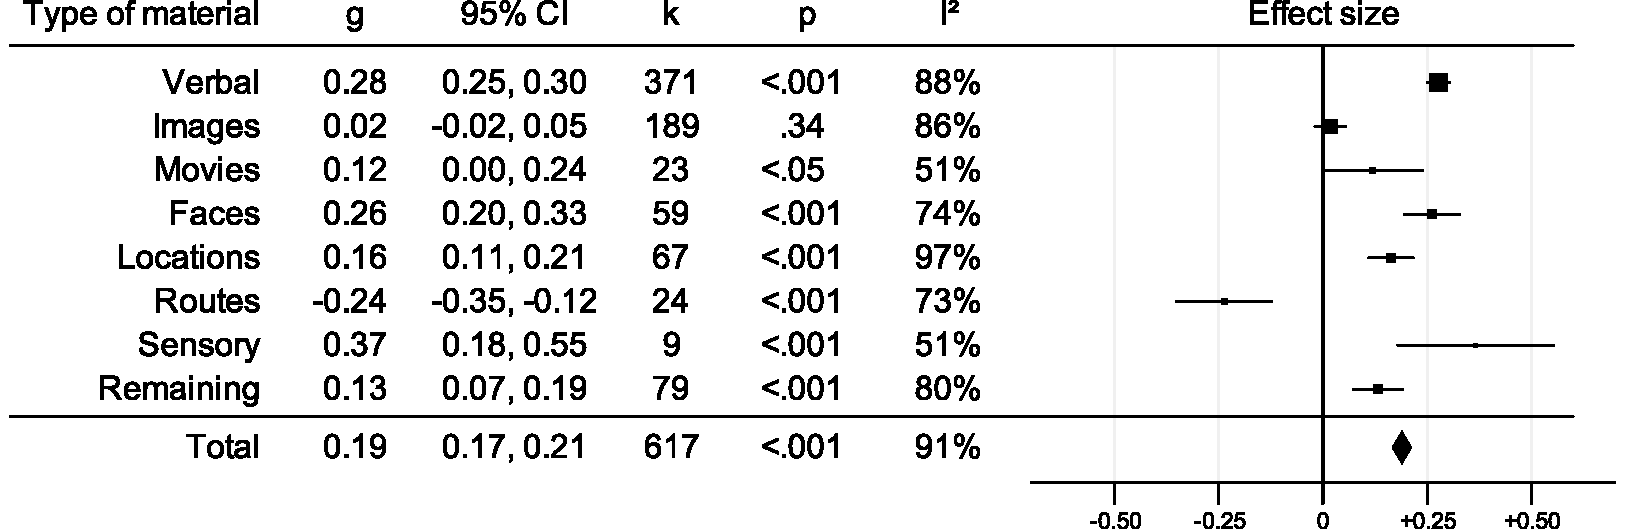
\includegraphics[width=120mm]{./Figures/Study1_TypeOfMaterial.pdf} \caption{Figure 2 from Study \Romannum{1} showing how the sex differences in episodic memory performance varies with the type of material that one is supposed to remember (Omnibus \emph{p}<.001; \emph{I}\textsuperscript{2}=89\%). Each row shows whether the effect size for that level of the moderator is reliably different from 0. The last row show the result from a meta-analysis without any moderators, performed on the full dataset. Positive values mean that women performed better than men. Explanation of headings: \emph{g} = Hedges' \emph{g}; 95\% \emph{CI} = the 95\% confidence interval; \emph{k} = number of studies; \emph{p} = the \emph{p}-value; \emph{I}\textsuperscript{2} = statistic denoting the percentage of variation across studies that is due to heterogeneity rather than due to chance.} \label{Figure:Study1_TypeOfMaterial} \end{figure}

Next, a number of moderator meta-analyses were performed at the task level, investigating each \emph{type of material} subset separately as well as the \emph{total} dataset. Here, the following moderators were investigated, which all had to do with aspects of the material to be remembered:

\begin{description} \item [Nameable material.] Whether the material was nameable, meaning that it could be remembered using verbal, mental representations.

\item [Emotional material.] Whether the material had a positive, negative, sexual, or neutral valence.

\item [Paired material.] Whether the material was paired with some other material and the participants were supposed to remember all the individual associations. \end{description}

Here, it was only the \emph{nameable material} variable that showed a somewhat consistent and interesting pattern (see Table 2 of Study \Romannum{1}): For the \emph{total} subset, women performed significantly better than men when the material was nameable (\emph{g}=0.14; \emph{p}<.001) and men performed significantly better than women when the material not was nameable (\emph{g}=-0.22; \emph{p}<.001). This was also the case for the \emph{images} subset where females performed significantly better on nameable images (\emph{g}=0.16; \emph{p}<.001) while men performed significantly better on non-nameable images (\emph{g}=-0.20; \emph{p}<.01). The effects went in the same directions, although not significantly so, for the two remaining subsets where this division was applicable: \emph{locations} (\emph{k}=29; omnibus \emph{p}<.20) and \emph{routes} (\emph{k}=19; omnibus \emph{p}<.24). These resuts further strengthen the expected pattern with regard to the verbal/spatial continuum.

Next, another set of moderator meta-analyses were performed, again at the task level and again investigating each \emph{type of material} subset separately as well as the \emph{total} dataset. This time, the moderators related to aspects of how the material was learned or retrieved:

\begin{description} \item [Repeated learning.] Whether the participants were given several chances to learn the material or simply had to remember it after just going through it once. \item [Intentional learning.] Whether the participants explicitly were asked to remember the material. \item [Retrieval support.] Whether the participants were asked to freely remember the material, remember the material with the help of one or more cues, or whether they recognized the material later presented to them. \item [Delayed recall.] Whether there was a delay between the presentation phase and the recall phase. \end{description}

Results (see Table 3 of Study \Romannum{1}) revealed no obvious and consistent patterns, but some interesting things can still be said: For \emph{repeated learning}, the subsets \emph{total}, \emph{verbal}, and \emph{images} showed significant omnibus tests, all going in the same direction with women increasing their performance more than men when repeating the material. However, the subset \emph{Routes}, which had a barely significant omnibus test (while the \emph{p} value is .05, it is rounded \emph{down} to this value), showed the opposite direction. If this possible pattern reflects something real in the population, it might simply be that whenever a group outperforms another for a certain type of material to be remembered, this advantage is even further increased when given a chance to repeat the material. As an analogy, imagine two persons trying to learn a new language, one of them being good at learning new languages, the other one being bad at it. After one week, some differences between the two should be seen, although not that large. On the other hand, after one year, the first one should be speaking the language fluently while the other one still probably speaks at a beginner level.

For \emph{retrieval support}, only the omnibus tests for the \emph{total} and the \emph{verbal} subset came out significant. Bear in mind that the overlap between these two sets always is very large though, in this case about 61\% of the data points in the \emph{total} set came from the \emph{verbal} subset, so whenever one of them shows a certain pattern, there is a good chance that the other one will as well. For both of these sets, women performed significantly better than men for recognition, which should be the easiest task, even better for cued recall, and finally with the largest margin for free recall, which should be the hardest task. This suggests a pattern where the excelling sex outperform the other sex more and more, the harder the task is. However, as mentioned, none of the other subsets had significant omnibus tests, and from just eyeballing the estimated effect sizes, no similar pattern can really be seen.

Next, a number of moderator meta-analyses were performed at the sample level, again investigating each \emph{type of material} subset separately as well as the \emph{total} dataset. More specifically, in addition to \emph{age}, \emph{sampling of subjects}, and \emph{year of publication} (that all were defined in section \ref{Moderators}), \emph{geographical region} was also investigated. This variable simply indicated where each study was carried out: Africa, Asia, Europe, North America, Oceania, or South America.

The results (see Table 4 of Study \Romannum{1}) showed, first of all, that \emph{geographical region} moderated the estimates within the two largest \emph{type of material} sets: \emph{verbal} and \emph{total}. This pattern was further investigated in Study \Romannum{3}. Further, \emph{sampling of subjects} could, due to unbalanced data, only be investigated for the \emph{verbal} and \emph{total} sets, where the omnibus tests were significant; in both cases, the females' performance was even larger than males for convenience-based samples compared to population-based samples. It is hard to say why this is the case, but it should be noted that all four (very large) open databases that were included were categorized as population-based. If these  somehow are different than the rest of the studies, they would most certainly impact the \emph{sampling of subjects} category. Most notably, they all utilize similar type of verbal memory tasks. None of the meta-regressions for \emph{year} came out significant, but for \emph{age}, relationships were present for \emph{verbal}, \emph{images}, and \emph{total} where both linear and quadratic regressions were fitted (see Figure 3 of Study \Romannum{1} for scatterplots and fitted regression curves for this data). While the effect was negative and linear for \emph{images}, the curve was parabolic for \emph{verbal}, implying that gender differences were somewhat smaller for younger and older persons than for the rest.

Finally, possible bias in the dataset was evaluated through four different moderator meta-analyses (with the moderators being defined in section \ref{Moderators}): \emph{database search} (whether data was taken from the first or second database search), \emph{data source} (whether data points were taken from publications or received from authors), and \emph{study objective} (whether sex differences explicitly were investigated). The results (see Table 1 of Study \Romannum{1}) showed no significant omnibus tests, meaning that no clear signs of bias in the dataset could be identified (for an extended discussion of this matter, see section \ref{Bias}).


In summary, I think that we, with this study, managed to give an exhaustive picture of what sex differences there are in episodic memory as well as which factors that are most important in order to understand the variation. More research can, of course, always be carried out, but I do not think that conducting another meta-analysis on this topic would be the best use of available resources.

\subsection{Study \Romannum{2}} \label{Variance_study}

Study \Romannum{2} is titled \emph{Sex Differences in Episodic Memory Variance}. It was published in \emph{Frontiers in Psychology} in 2020 \parencite{Asperholm2020}.

\subsubsection{Introduction}

As already briefly outlined in section \ref{Research_questions}, the goal of study \Romannum{2} was to investigate variance differences between men and women in episodic memory performance, mainly with regard to the type of material to be remembered. Here, it was hypothesized that in line with previous research on sex differences in both cognition and more general traits (see section \ref{Variance_differences}), men would be more variable on both the full dataset as well as for all material categories.

\subsubsection{Method}

For this study, several five-level meta-analyses (further described in section \ref{Statistics} and \ref{Dependency}) were conducted on a subset of the original dataset (the full dataset is described in section \ref{Dataset}, and the subset is described further down), using the dependent variables Hedges' \emph{g}/\emph{lnVR} and the weighted variance of Hedges' \emph{g}/\emph{lnVR} (further described in section \ref{Effect_sizes}).

For these analyses, only data points where some kind of variance metrics were presented separately for men and women could be used (for example, if only pooled standard deviation was available for a data point, that data point had to be discarded). This resulted in a final dataset where 535 out of the 617 studies in the full dataset were included, totaling 962,946 participants.

\subsubsection{Results and discussion}

First, we performed a replication of an analysis in Study \Romannum{1} (see Figure \ref{Figure:Study1_TypeOfMaterial}) with Hedges' \emph{g} as the dependent variable and \emph{type of material} to be remembered as the moderator. This was carried out in order to make sure that the original results from Study \Romannum{1} still held for the somewhat reduced dataset. Results (see Table 1 in Study \Romannum{2}) showed that the categories \emph{movies} and \emph{remaining} went from being significant to non-significant.

Next, the same analysis as above but with \emph{lnVR} as the dependent variable was carried out. The results (see Figure \ref{Figure:Study2_Type_of_material}) showed that men were more variable for \emph{verbal} and \emph{locations}, while women were more variable for \emph{routes}. Men were also more variable for the \emph{total} dataset. What is interesting to note here is that when comparing the results of the \emph{type of material} moderator analyses using Hedges' \emph{g} as the dependent variable to the same analyses using \emph{lnVR} as the dependent variable, it can be seen that they mirror each other for all level pairs that are significantly different from zero in both analyses. That is, whenever women performed better than men, men also had larger variance than women and vice versa (I will come back to this shortly).

\begin{figure} \centering 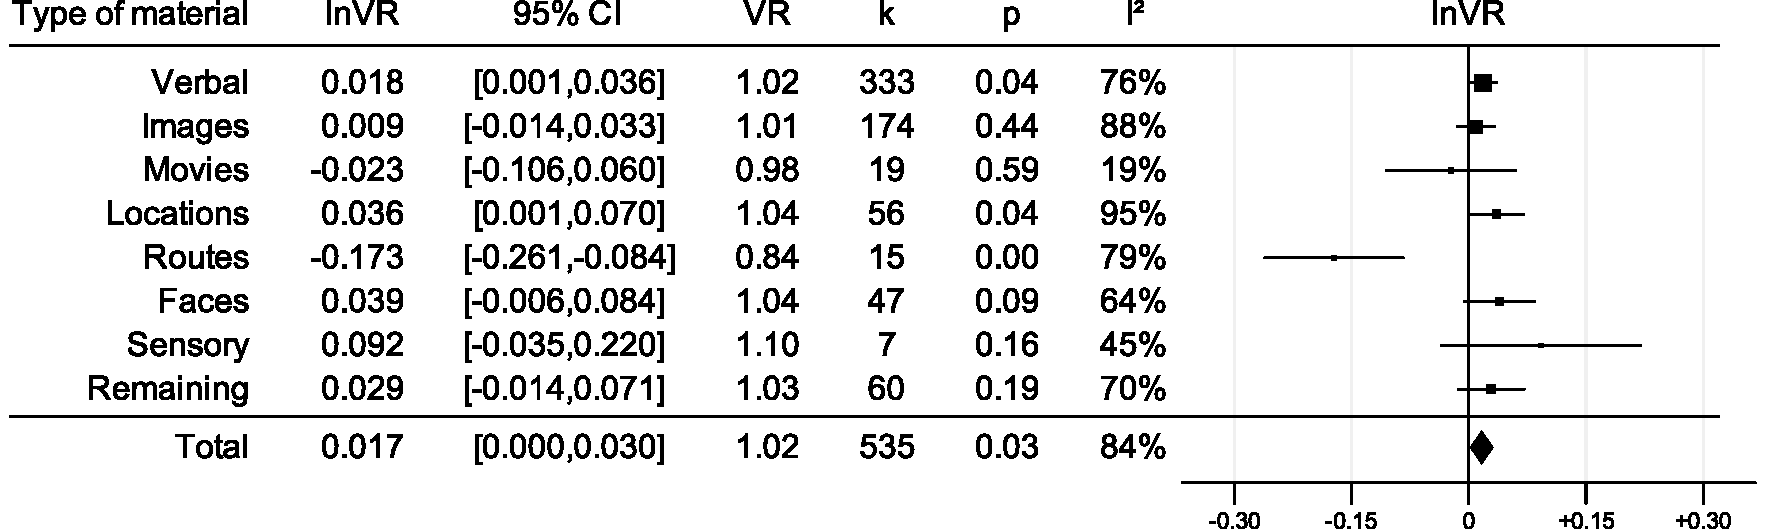
\includegraphics[width=120mm]{./Figures/Study2_Type_of_material.pdf} \caption{Figure 2 from Study \Romannum{2} showing how the variance sex differences in episodic memory performance varies with the type of material that one is supposed to remember (Omnibus \emph{p}<.01;  \emph{I}\textsuperscript{2}=83\%). Each row shows whether the effect size for that level of the moderator is reliably different from 0. The last row show the result from a meta-analysis without any moderators, performed on the full dataset. Positive values mean that women performed better than men. Explanation of headings: \emph{lnVR} = \emph{lnVR}; 95\% \emph{CI} = the 95\% confidence interval; \emph{k} = number of studies; \emph{p} = the \emph{p}-value; \emph{I}\textsuperscript{2} = statistic denoting the percentage of variation across studies that is due to heterogeneity rather than due to chance.} \label{Figure:Study2_Type_of_material} \end{figure}

Further, we performed a number of meta-regressions with either \emph{age} or \emph{publication year} (defined in section \ref{Moderators}) as moderators on each \emph{type of material} subset as well as on the \emph{total} dataset. Results (see Table 2 and Table 3 in Study \Romannum{2}) showed that \emph{publication year} had no effect on the outcome. Further, for \emph{age}, two small, negative linear relationships could be found, here indicating that the men's larger variances compared to women became smaller across age.

Next, a number of meta-analyses were carried out in order to search for possible bias in the dataset, using the following four moderators (defined in section \ref{Moderators}): \emph{database search} (whether data was taken from the first or second database search), \emph{data source} (whether data points were taken from publications or received from authors), \emph{study objective} (whether sex differences explicitly were investigated), and \emph{sampling of subjects} (whether the sample was convenience-based or population-based). Similarly to Study \Romannum{1}, only \emph{sampling of subjects} showed a significant omnibus test (see Table 4 of Study \Romannum{2}), meaning that the sex difference in variance was more positive (that is, towards men having larger variance) in convenience-based samples compared with population-based samples. Otherwise, there were no indications of bias in the dataset. As already mentioned in the results section of Study \Romannum{1}, all data from the open databases were categorized as population-based, which means that possible deviations in these have a large probability of showing up for the \emph{sampling of subjects} variable as well.

Returning to what was discussed earlier, a somewhat interesting and consistent, mirrored pattern appeared when comparing the two \emph{type of material} moderator analyses performed with Hedges' \emph{g} and \emph{lnVR} as dependent variables respectively: That is, whenever men performed better for a material category, women also had larger variance than men and vice versa. This pattern was further investigated in a number of exploratory meta-regressions performed separately for all the \emph{type of material} subsets as well as the \emph{total} dataset, where \emph{lnVR} was set as the dependent variable and Hedges' \emph{g} as a moderator. Results (see Table 5 in Study \Romannum{2}) showed significant, positive relationships for the \emph{verbal}, \emph{images}, \emph{locations}, \emph{routes}, \emph{faces}, and \emph{total} sets, and a significant, negative relationship for the \emph{sensory} subset. That is, there were positive relationships found between the mean differences and variance differences for all categories where the mirrored pattern described above could be identified. A positive relationship here indicates that as the performance goes toward favoring women on a given task, the variance of men becomes larger and larger compared to the women's and vice versa (for an illustration of this relationship for the full dataset, see Figure \ref{Figure:Study2_lnVR_g_relationship}).

\begin{figure} \centering 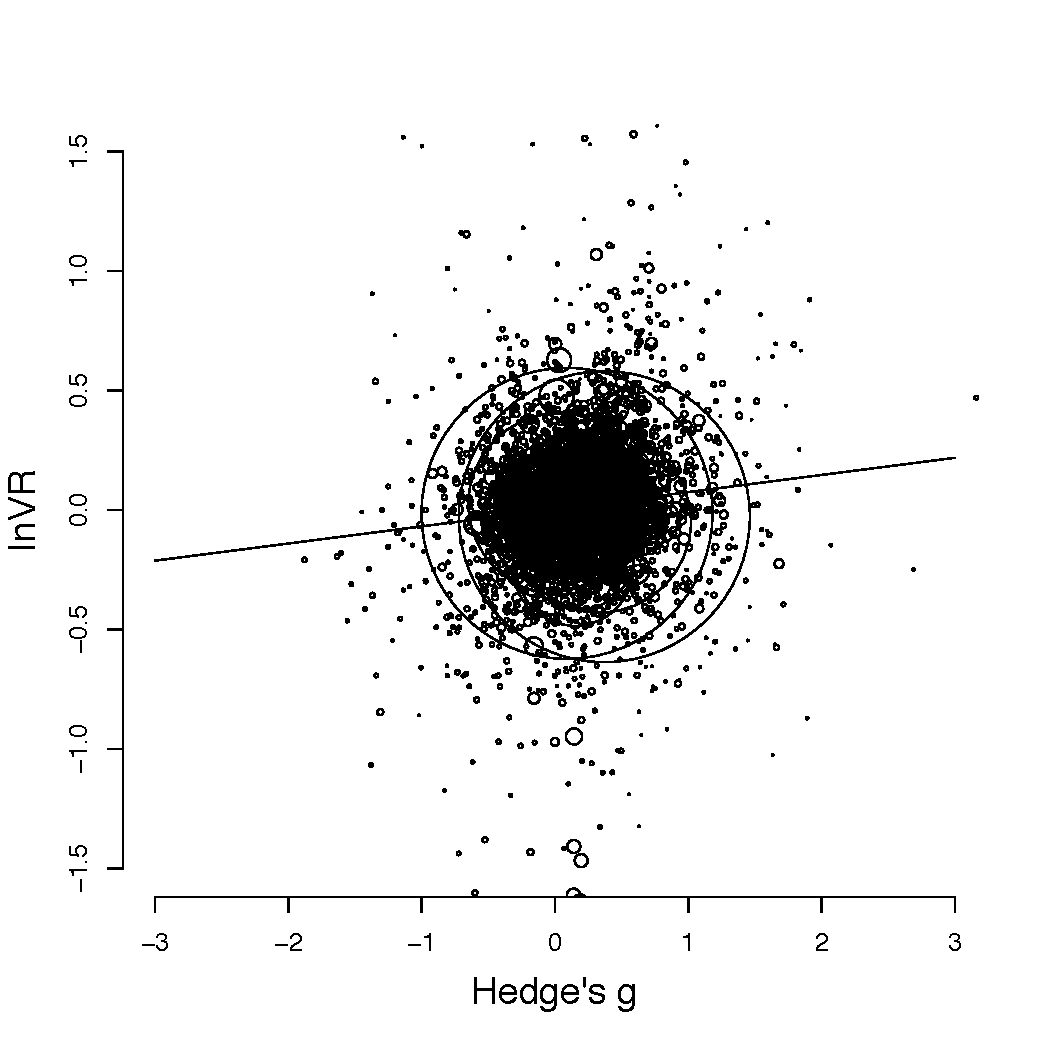
\includegraphics[width=120mm]{./Figures/Study2_lnVR_g_relationship.pdf} \caption{Figure 3 from Study \Romannum{2} showing the relationship between \emph{lnVR} (where positive values mean that males have more variance than females) and Hedges' \emph{g} (where positive values mean that females perform better than males) for the full dataset. The diameter of each data point is equal to the inverse of its squared weighted variance (see section \ref{Statistics} for an explanation of this concept). The drawn line shows the best-fitting regression line from the significant meta-regression reported in Table 5 of Study \Romannum{2}.} \label{Figure:Study2_lnVR_g_relationship} \end{figure}

One way of explaining this pattern could be that it comes about because of ceiling effects. That is, when one sex performs much better than the other, they may also hit a ceiling, either an actual limit to their performance or an upper bound resulting from how the test is designed; an example of the former being if they were asked to recall fewer items than what they actually were capable of remembering. Since the performance distribution (regardless of the underlying reason for this ceiling effect) then would be restricted for the top achievers, the variance would also become narrower. This, in turn, would mean that the sex who would be less affected by this ceiling effect also would have larger variance than the other.

If a ceiling effect like the one described above would come about because of an actual limit in the cognitive performance, this would also reflect an actual difference in the variance between men and women. Such a limit --- or diminishing returns effect if you will --- is something that is bound to happen at some point if the performance of one sex keeps increasing in relation to the other, the question is only when. However, if it would come about because of deficiencies in how the outcome was measured, the obtained results would only be artifacts, not indicating a real phenomenon in the underlying performance. With the data we have, finding out which of these factors contribute to the outcome to what degree (if at all) is not possible. However, it \emph{is} possible to point to other large studies where the mean and variance differences go in the same direction \parencite{Hedges1995, Machin2008, Nowell1998, Lakin2013}, indicating that \emph{even if} a ceiling effect could be a factor in some cases, it cannot fully explain why men seem to be more variable than women in many areas.

Finally, an illustration of what the overall distributions for men and women would look like, given that the estimations from the two \emph{type of material} moderator analyses presented above were accurate, is shown in Figure \ref{Figure:Study2_Assumed_distributions}. Here, while it can be argued that the variance differences are quite small, it can also be seen that the distributions of men and women in the extremes are not negligible. For example, for the \emph{verbal} category, there are 1.76 women for each man in the top 5\%.

\begin{figure} \centering 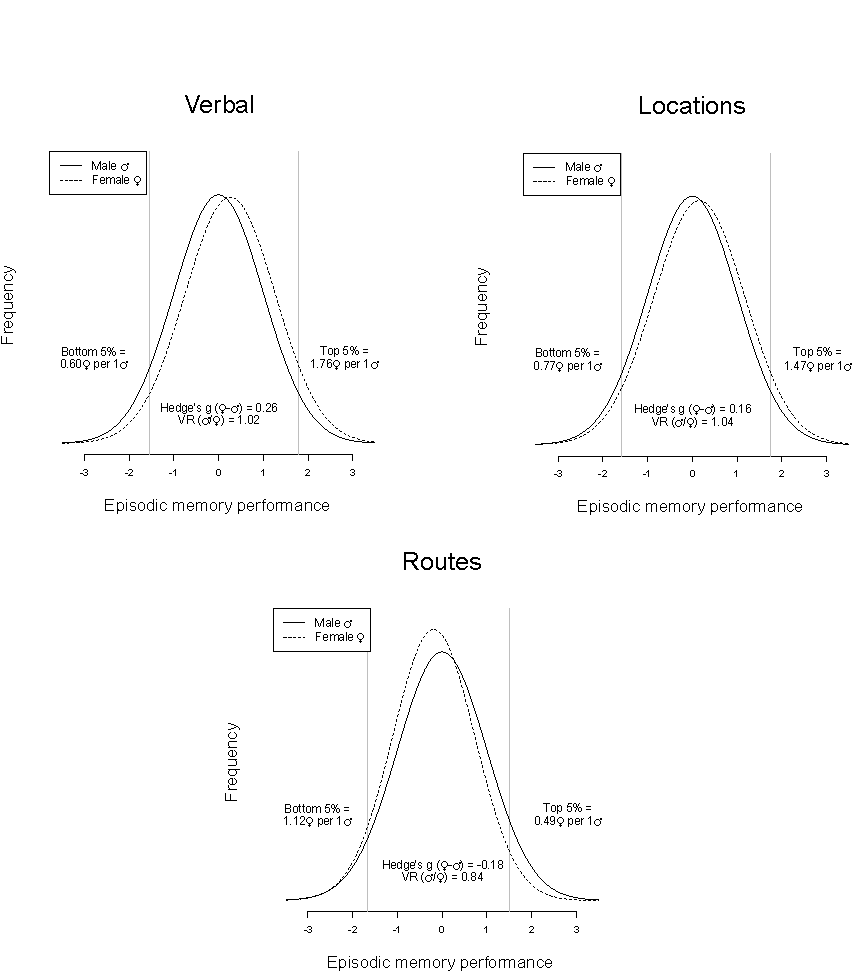
\includegraphics[width=120mm]{./Figures/Study2_Assumed_distributions.pdf} \caption{Figure 4 from Study \Romannum{2} that shows assumed distributions of male and female performance for the \emph{verbal}, \emph{locations}, and \emph{routes} subsets. These distributions are computed based on the estimates of Hedges' \emph{g} and \emph{lnVR} in the respective analyses where these were assessed with \emph{type of material} as a moderator (see Table 1 of Study \Romannum{2} and Figure \ref{Figure:Study2_Type_of_material} of this thesis). Assumed distributions are only shown for \emph{type of material} categories where both of these estimates significantly differed from zero.} \label{Figure:Study2_Assumed_distributions} \end{figure}

In summary, the small effect sizes that were shown combined with some question marks surrounding possible ceiling effects in the underlying data makes this study informative but also warrants further research. More specifically, it would probably be useful to investigate a large dataset containing the raw participant data, rather than just descriptive summary statistics, meaning that it would be possible to say more about potential problems in it. Even so, the study does provide some circumstantial evidence that what has already been shown for other domains, namely that males tend to vary more as a group than females, also might be the case for episodic memory.

\subsection{Study \Romannum{3}} \label{Social_study}

Study \Romannum{3} is titled \emph{The Magnitude of Sex Differences in Verbal Episodic Memory Increases with Increased Gender Equality: Data from 54 Countries Across 40 Years}. It was published in \emph{PLOS ONE} in 2019 \parencite{Asperholm2019b}.

\subsubsection{Introduction}

As already briefly outlined in section \ref{Research_questions}, the goal of study \Romannum{3} was to investigate if men and women are affected differently by societal progression when it comes to mean differences in episodic memory performance. More specifically, we first wanted to explore whether country moderated the mean sex difference effect in episodic memory performance. If this would be the case, we then wanted to go on and investigate possible predictors that could make sense of this pattern. The hypothesis was that country would moderate the mean sex difference effect and that social progress would be positively related with changes in sex differences to women's adgantage. Further, we hypothesized, in line with earlier research (see section \ref{Variance_differences_Episodic_memory}), that a measure of gender equality would be the strongest social progress predictor for this relationship among the measures investigated.

\subsubsection{Method}

For this study, we used the dataset described in section \ref{Dataset}. However, only studies that had been performed within a single, known country were included, resulting in a final dataset of 612 studies, originating from 54 different countries, published between 1973 and 2013, and involving a total of 587,691 participants. Further, the dataset was divided into \emph{verbal} and \emph{non-verbal} material. Here, \emph{verbal} material was defined the same way as in the \emph{type of material} variable (see section \ref{Moderators}), with the addition that nameable images (see section \ref{Study1_Method}) also were included. This decision was made in light of the results of Study \Romannum{1}, where women did not only perform better than men for nameable images, but where there also was a significant difference between nameable images and non-nameable images. In addition to their theoretical closeness, this made nameable images similar to the verbal material category from an empirical standpoint as well; when remembering words, they can often be remembered as images, and vice versa.

Further, three indicators of social progress were constructed, where each unique country and year combination received a value based on what the numbers were at that specific point in time for that specific country. Data for these measures were taken from \emph{\citeauthor{UNDP}} (UNDP) and \emph{\citeauthor{WB}} (WB). The three indicators were defined as follows:

\begin{description} \item [Gender Equality.] A composite measure that was made up of (1) the UNDP indicator \emph{Average Years of Schooling Attained (Female population, 25 years and over)} subtracted by \emph{Average Years of Schooling Attained (Male population, 25 years and over)} and (2) the WB indicator \emph{Female to male ratio on labor force participation (for ages between 15 and 64)}. \item [Population education and employment.] A composite measure that was made up of (1) the UNDP indicator \emph{Average Years of Schooling Attained (Total population, 25 years and over)} and (2) the WB indicator \emph{Labor force participation rate (\% of total population ages 15-64)}. \item [GDP per capita.] Gross domestic product per capita is a measure of economic activity in relation to the size of the population. This measure, given in current US dollars, was extracted from the WB database and subsequently transformed using the natural logarithm to achieve a normal distribution of the variable. \end{description}

Indicators were not always available for every year. Whenever an indicator was missing, it was extrapolated from indicator values surrounding it. Further, each indicator was z-transformed using the full distribution of all possible year and country combinations for the included countries between 1972 to 2013. Also, correlation analyses for the full dataset revealed positive associations between the three indicators (\emph{Gender Equality} vs. \emph{Population Education and Employment}: \emph{r}=.70, \emph{p}<.001; \emph{Gender Equality} vs. \emph{GDP per Capita}: \emph{r}=.50, \emph{p}<.001; \emph{Population Education and Employment} vs. \emph{GDP per Capita}: \emph{r}=.56, \emph{p}<.001).

When it comes to indicators measuring different types of social progress and living conditions constructs, such as the ones presented above, there are a lot of choices to be made. For example, one of the most popular measures with regard to gender equality is the \emph{Global Gender Gap Index} (GGGI) \parencite{WEF2020}. This is a composite measure consisting of a number of variables that together are meant to gauge women's opportunities/participation when it comes to economy, politics, health and education. However, it can be questioned whether this scale actually captures gender equality, and other measures have been proposed \parencite{Stoet2019}. One critique here is, for example, that within the scope of the GGGI, it is theoretically impossible for women to be better off than men because underlying measures are capped once they reach perfect symetry between the sexes. It also does not focus on areas where men usually are worse off such as harsher punishments when it comes to crime, higher suicide rates, and more occupasional accidents \parencite{Stoet2019}.\footnote{However, it can, of course, also be questioned to what extent actual outcomes measures oppurtunities. Does low policital participation from women automatically mean that they are held back? Does higher suicide rates for men mean that society somehow has done something wrong?}

For the present study, we needed to find indicators that not only captured the underlying concepts that we were interested in, but also that suited our data fairly well when it comes to available data for the specific countries and year that we happened to need. As such, we chose to go with the relatively simple measures specified above.

\subsubsection{Results and discussion}

First, in order to evaluate whether country moderated the episodic memory effect size, two five-level meta-analyses with country as a moderator were performed, one on the \emph{verbal} subset and one on the \emph{non-verbal} dataset. Results (see Figure \ref{Figure:Study3_Figure1}) showed that for the \emph{verbal} subset, country was significantly modifying the effect sizes. However, for the \emph{non-verbal} subset, it did not. Therefore, going further, only the \emph{verbal} subset was considered.

\begin{figure} \centering 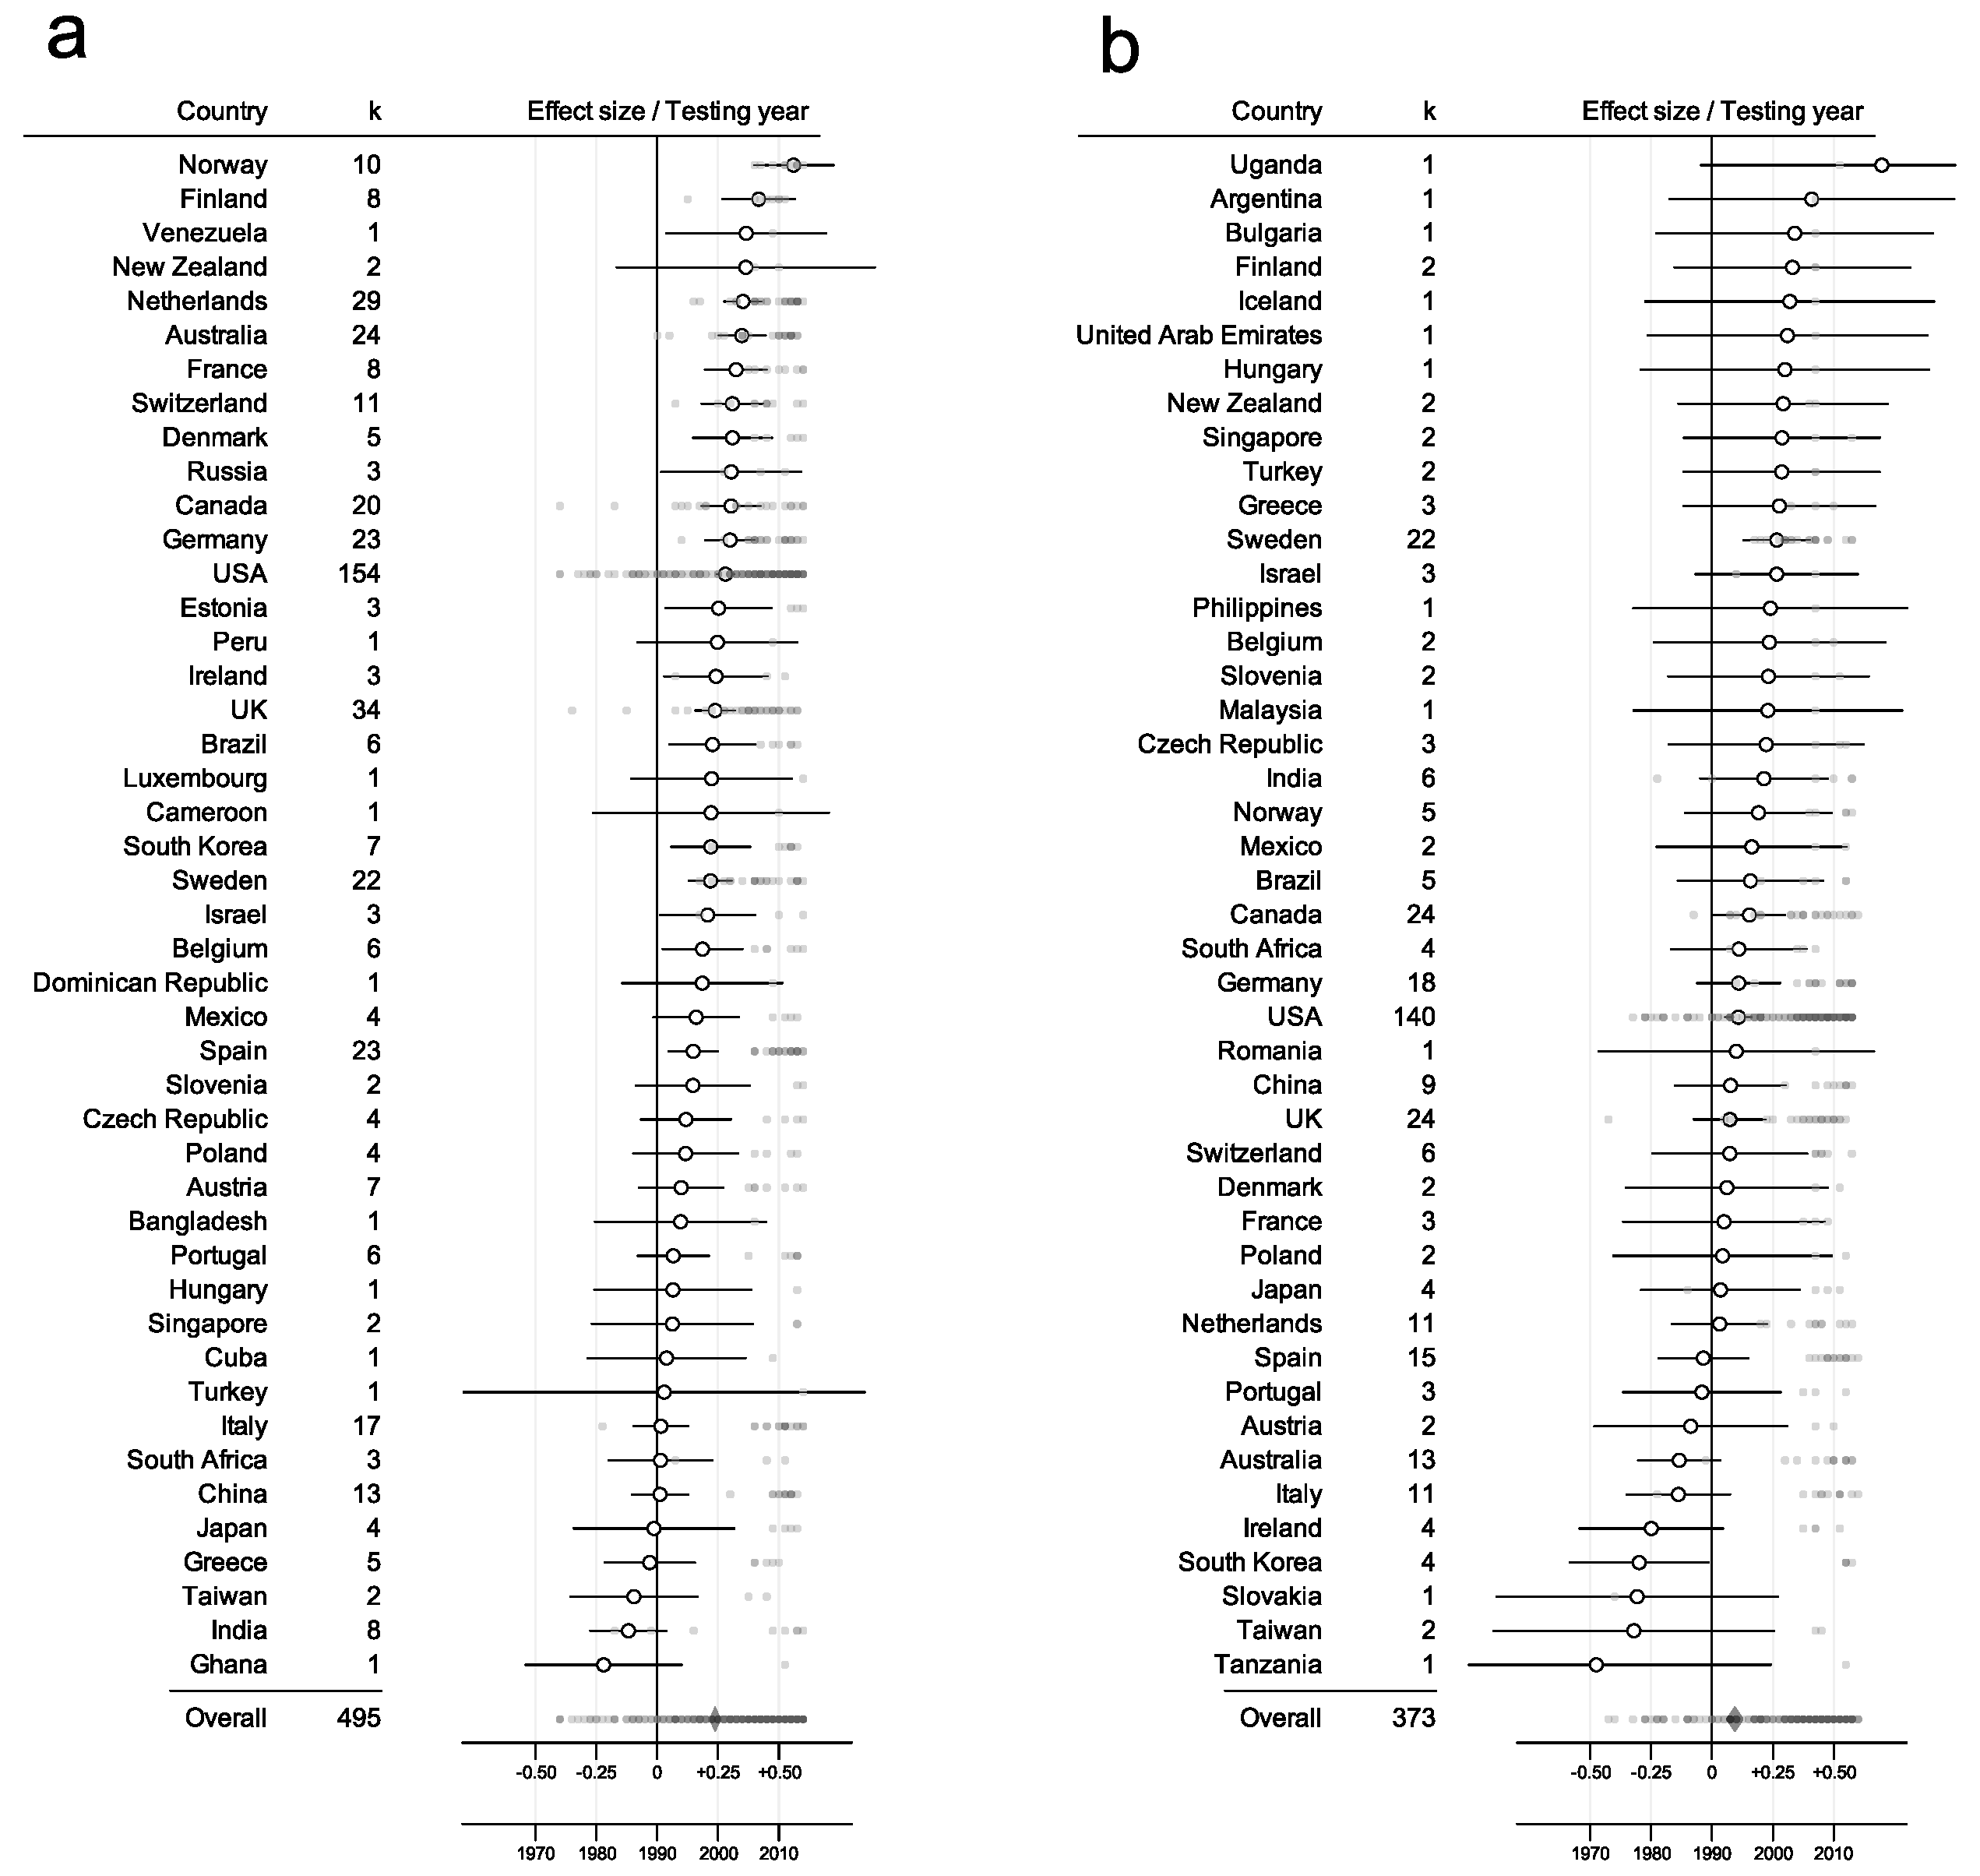
\includegraphics[width=120mm]{./Figures/Study3_Figure1.eps} \caption{Figure 1 from Study \Romannum{3} (taken from the correction of the original article; \citeauthor{Asperholm2019c}, \citeyear{Asperholm2019c}) showing the results of two moderator analyses (investigating the \emph{verbal} and \emph{non-verbal} sets of the data) with country as a moderator and Cohen's \emph{d} of episodic memory performance as the dependent variable. Number of studies is indicated by the \emph{k} column. Positive values indicate that women perform better than men.} \label{Figure:Study3_Figure1} \end{figure}

Next, we fitted a number of six-level meta-analyses (where country was added as the sixth level on top of the hierarchical structure described in section \ref{Hierarchical_structure}): The first thing we did was to fit three simple models with each of the social progress indicators as moderators and then a combined model with all three of them included simultaneously. Here, Cohen's \emph{d} of episodic memory performance along with the weighted variance of Cohen's \emph{d} were the dependent variables, and each effect size was paired with the right social progress indicator value according to when\footnote{Here, we used the publishing year of the article in question minus one to better reflect when the experiment in the study probably was carried out. Just subtracting by one was probably too conservative though, and in retrospect I believe that we could have increased this number. I also believe that this would not affect the overall results.} and where the study was carried out. The results (see Table \ref{Table:Study3_Meta-regressions}) of the three simple regressions all showed significant, positive relationships between the dependent variable and the indicator (see Figure \ref{Figure:Study3_Figure2} for illustrations of these effects). That is, they all went in the expected direction where an increase in women's relative episodic memory performance compared to men's was related to increased social progress. However, for the combined model, comprising all three social progress indicators, a significant, positive relationship could only be found for \emph{Population Education and Employment}. Here, one \emph{z}-point change for this indicator was associated with an increase of 0.08 in Cohen’s \emph{d} for verbal episodic memory performance.

\begin{table} \caption{Adapted version of Table 1 in Study \Romannum{3} showing summary statistics of the four meta-regression analyses (SM = Simple model; CM = Combined model) for \emph{verbal} episodic memory performance. Explanation of symbols: $*\rightarrow$ \emph{p}<.05; $**\rightarrow$ \emph{p}<.01; $***\rightarrow$ \emph{p}<.001. Notice that there is a typo in the original article that has been corrected here: The \emph{Gender Equality B} estimate for SM1 should be \emph{p}<.001 rather than \emph{p}>.05.} \label{Table:Study3_Meta-regressions} \centering
\small
\begin{tabular}{lcccc}
\toprule
                                            & SM1                         & SM2                       & SM3                       & CM                        \\ \midrule
  Intercept                                 &                             &                           &                           &                           \\
  \hspace{10mm} Estimate                    & 0.16\textsuperscript{***}   & 0.13\textsuperscript{***} & 0.18\textsuperscript{***} & 0.14\textsuperscript{***} \\
  \hspace{10mm} Standard error              & 0.02                        & 0.02                      & 0.02                      & 0.02                      \\
  Gender Equality                           &                             &                           &                           &                           \\
  \hspace{10mm} B estimate                  & 0.10\textsuperscript{***}   &                           &                           & 0.04                      \\
  \hspace{10mm} B standard error            & 0.02                        &                           &                           & 0.03                      \\
  Population E\&E                           &                             &                           &                           &                           \\
  \hspace{10mm} B estimate                  &                             & 0.13\textsuperscript{***} &                           & 0.08\textsuperscript{*}   \\
  \hspace{10mm} B standard error            &                             & 0.02                      &                           & 0.04                      \\
  GDP per Capita                            &                             &                           &                           &                           \\
  \hspace{10mm} B estimate                  &                             &                           & 0.60\textsuperscript{***} & 0.18                      \\
  \hspace{10mm} B standard error            &                             &                           & 0.16                      & 0.20                      \\
  Observations                              & 2681                        & 2681                      & 2681                      & 2681                      \\
  R\textsuperscript{2}                      & 0.12                        & 0.15                      & 0.11                      & 0.16                      \\ \bottomrule
\end{tabular}
\normalsize
 \end{table}

\begin{figure} \centering 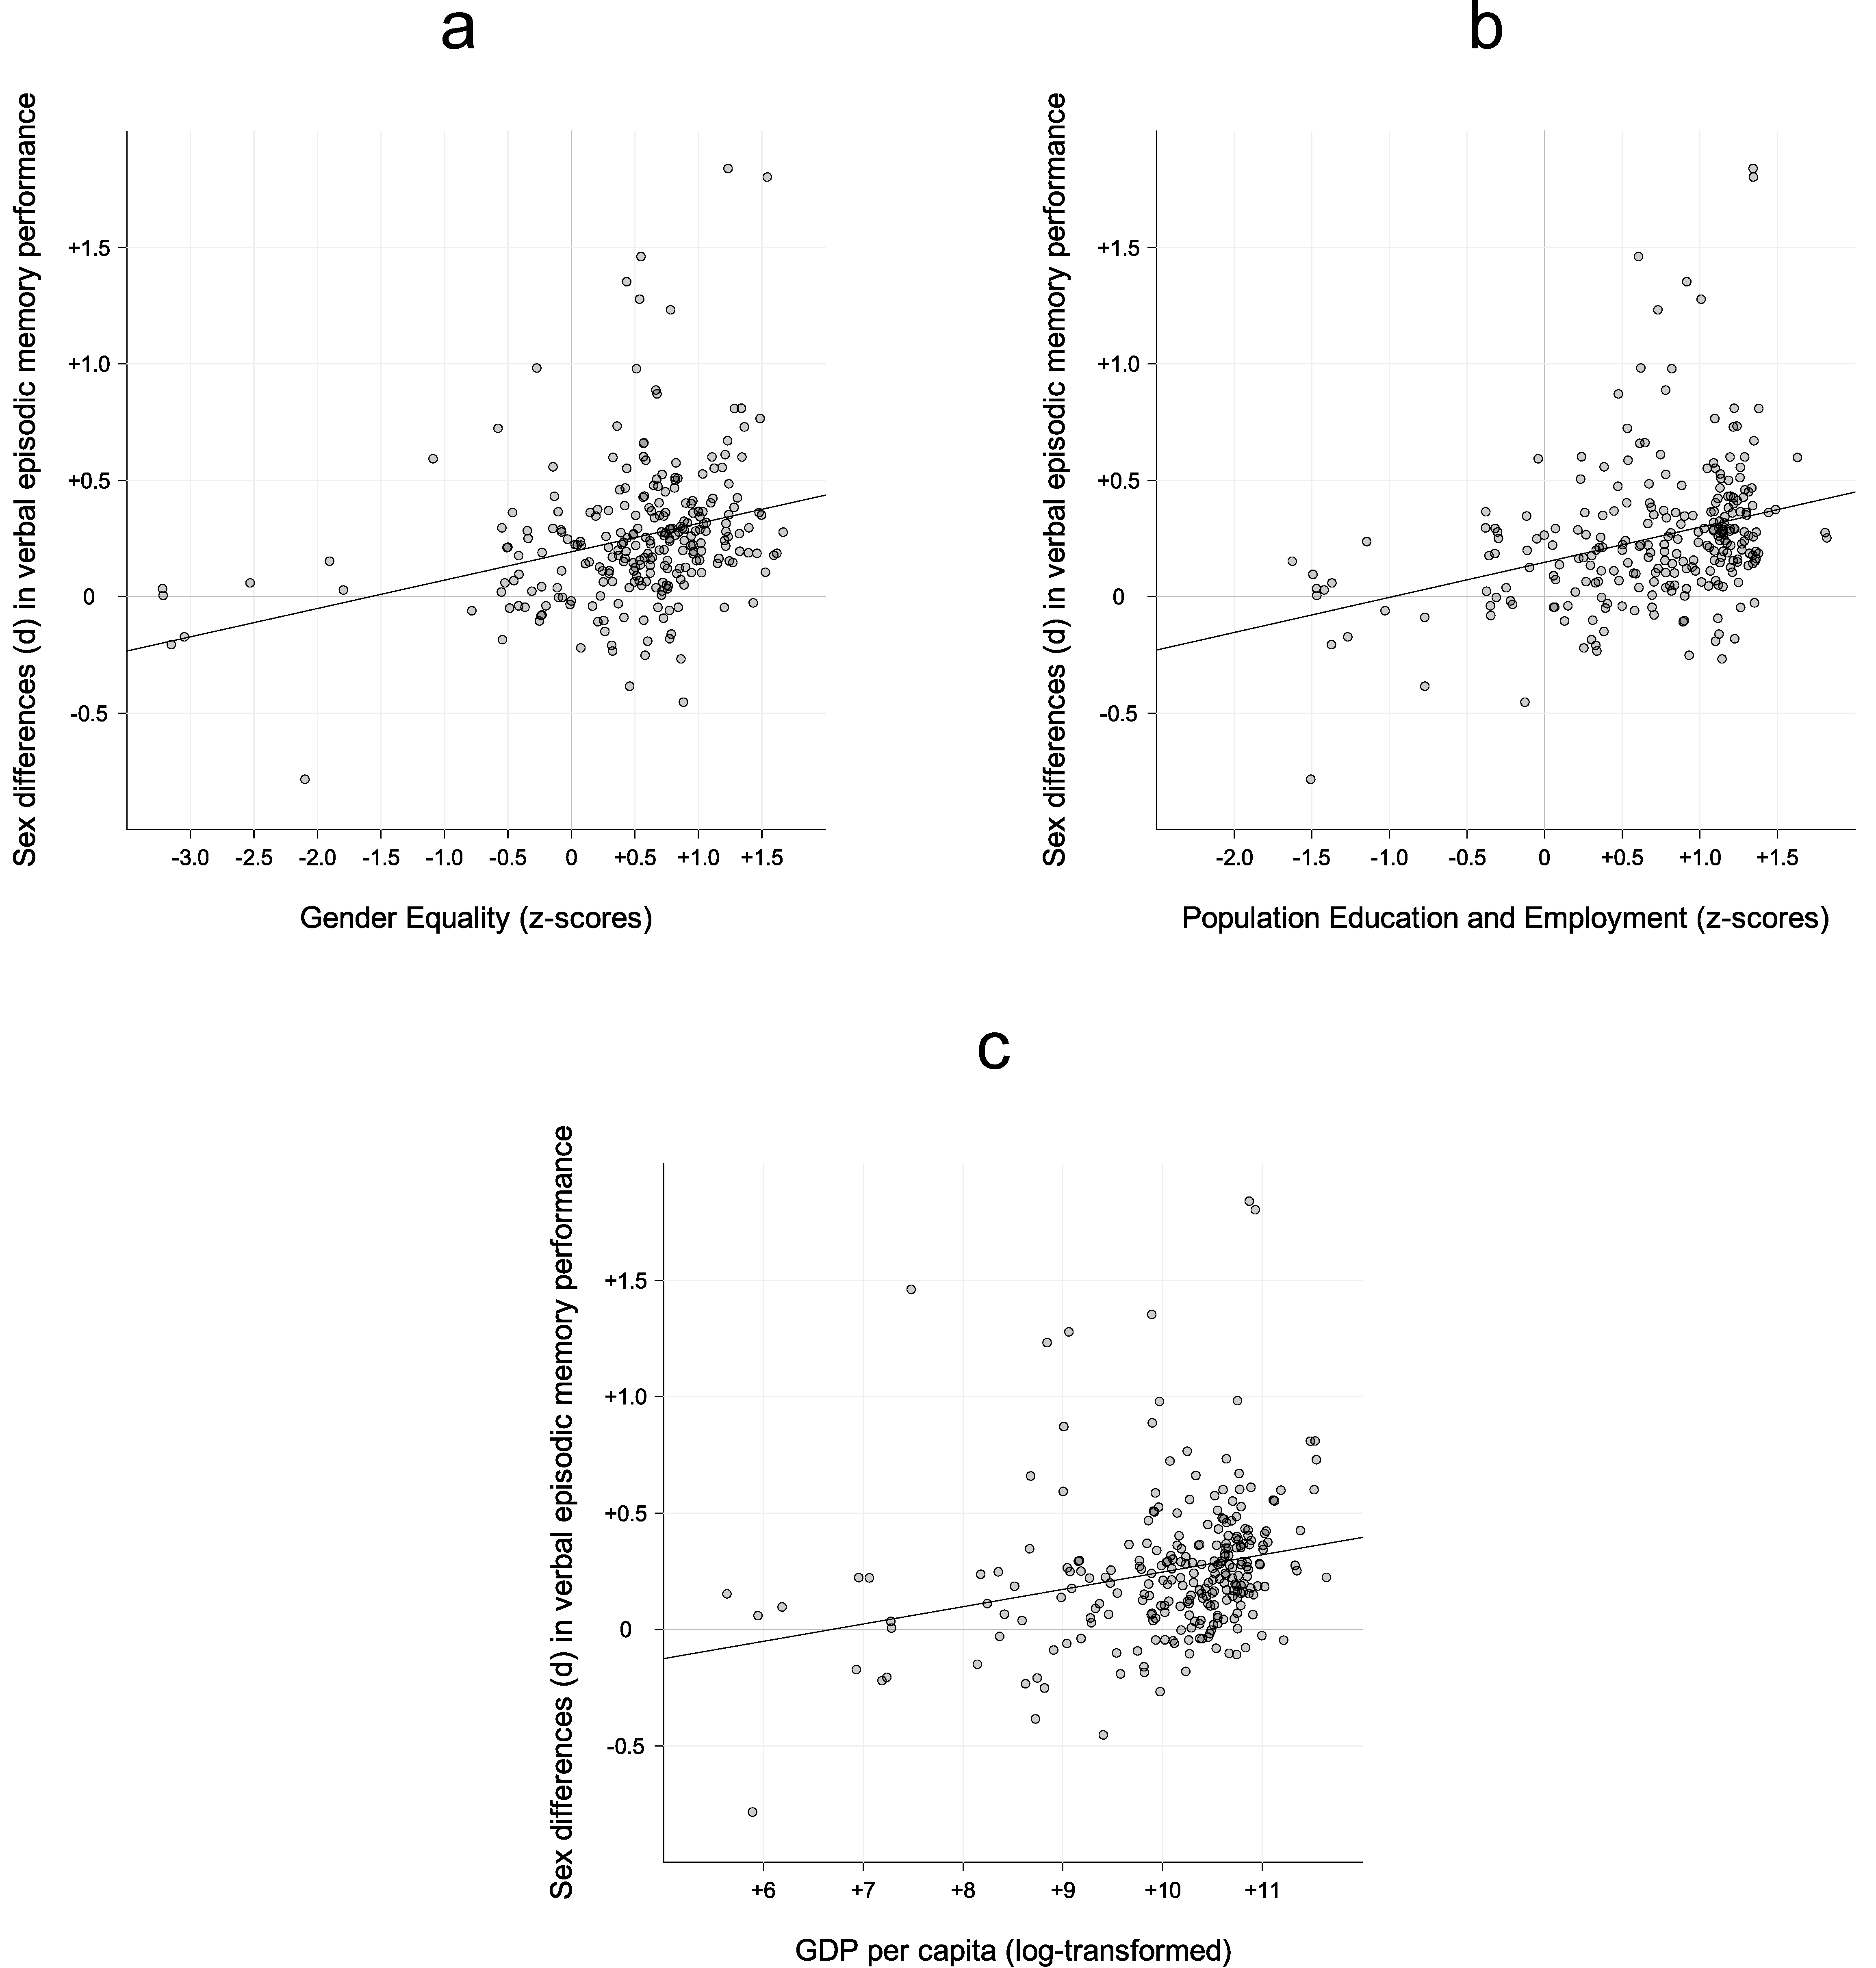
\includegraphics[width=120mm]{./Figures/Study3_Figure2.pdf} \caption{Figure 1 from Study \Romannum{3} (adapted from the correction of the original article; \citeauthor{Asperholm2019c}, \citeyear{Asperholm2019c}) showing the best-fit regressions of the three separate meta-regressions with sex difference in \emph{verbal} episodic memory performance as the dependent variable and the social progress indicators (a) \emph{Gender Equality}, (b) \emph{Population Education and Employment}, and (c) \emph{GDP per Capita} as continuous moderators.} \label{Figure:Study3_Figure2} \end{figure}

In addition, we performed the same meta-regressions as above for \emph{verbal} episodic memory tasks, both \emph{without} the large databases that were the sole focus for \textcite{Weber2014} and \textcite{Bonsang2017} as well as with \emph{only} these databases. This did not change the outcome in a major way (see S2 Table of Study \Romannum{3}). For the analysis without the databases, \emph{Population Education and Employment} went from being significant to marginally significant for the combined model. For the analyses with only the databases, \emph{GDP per capita} went from not being significant to actually being significant.

The upshot of the results of this study is that while all social progress indicators tested for could be shown to be positively related to women's relative increase in verbal episodic memory performance compared to men's, it was the overall education and employment level rather than the gender equality level that best predicted this. Given the reasoning laid out in section \ref{Societal_explanation} --- where it is argued that increases in living standards should benefit women more since men might experience a form of diminishing returns effect from already having access to more social goods --- it would make sense that increasing the general level of education and employment, independent of sex, could benefit women more than men as long as they were not left out completely.

It is also possible to construct a hypothetical scenario showing how gender equality could be less important: Imagine two countries, Oceania and Eurasia. In Oceania, the general standard of living has increased dramatically while gender equality has seen less progression. In Eurasia, the general standard of living has been quite unimpressive while gender equality has seen a striking improvement. In this scenario, women in Oceania would probably experience larger increases in cognitive performance compared to men than what women in Eurasia would. If our dataset were to share characteristics with this example, it could be argued that this at least in part could explain the pattern seen.

In summary, with this study, we have further strengthened what others already have suggested, namely that social progress is related to relative improvements in sex differences to women's advantage, both in cognition in general and for episodic memory. However, the fact that it was the overall education and employment level rather than the gender equality for these measures that was the best predictor for the outcome suggests that more in-depth studies, probably applying some other method than what has been used so far, are needed in order to better explain what is going on.

\section{Discussion}

For this thesis, I have through three different studies investigated sex differences in episodic memory from several, disparate perspectives. Rather than setting up experiments and gathering participant data ourselves, we synthesized and combined already produced data in order to reach new and powerful conclusions.

In Study \Romannum{1}, we performed a meta-analysis on mean sex differences in episodic memory, using a dataset of 617 studies that we compiled for this purpose, consisting of both published and unpublished data, as well as several open databases. Here, we could first and foremost, as expected, see a strong indication that just like with other cognitive tasks, the difference in performance between men and women depends on what type of material they are being exposed to. More specifically, men tend to perform better on more spatial tasks while women tend to perform better on more verbal tasks, and this pattern also seems to be in place for episodic memory. Women also performed better than men for tasks having to with remembering faces as well as assignemtns pertaining to smell, touch, and different shades of colors. These type of tasks cannot, at least not on the face of it, be categorized as either verbal or spatial and would therefore suggest a broader advantade for females when it comes to episodic memory.

In Study \Romannum{2}, we performed a number of analyses on the same dataset gathered in Study \Romannum{1}, searching for variance differences between men and women. Here, we could, in line with our expectations as well as previous research, find that men overall were slightly more variable than women when it comes to episodic memory. However, we also found some exploratory results that implied that those findings might come about because of underlying methodological problems in the original research, more specifically possible ceiling effects in a subset of the tasks. Therefore, more research to investigate these potential problems is warranted.

In Study \Romannum{3}, we performed a number of analyses on the same dataset gathered in Study \Romannum{1}, investigating whether sex differences were related to social progress. Here, we could first see that which country a study was conducted in also affected the sex difference in verbal episodic memory. Investigating this further, we concluded that sex differences in verbal episodic memory tracked several different indicators of social progress tied to the year and country of each individual study. However, when pitted against each other, it was only the education and employment level that could be shown to have an effect and not gender equality, which we expected would be the most important indicator.

It should be mentioned that while the sex differences and effects that are demonstrated within the scope of these three studies often are quite small, one should keep in mind that they also represent basic cognitive skills that form the basis of a plethora of higher-order cognitive functions. In that respect, it is not unreasonable to suspect that these small differences will be amplified and result in much more obvious differences for more complex behaviors. For example, when reading a text, episodic memory is involved for multiple tasks that you have to carry out, for example encoding what you currently are reading, recalling what you read previously, as well as remembering newly defined terms and concepts. This means that performing just slightly better in episodic memory also will impact all of these tasks which in all individually increases the overall reading performance. When combining this with repeated exposures and training over a long time, even small effects for basic skills should translate to larger effects for more composite skills.

I will now turn to discuss some general aspects of the studies included in this thesis more in-depth.

\subsection{Quality vs. quantity}

When collecting a large amount of data in order to get a full picture of the research that has been done within a field (as we did for the studies in this thesis), one often has to make a sort of quality/quantity decision. That is, on the one extreme, for our data collection we could have chosen a single standardized test of episodic memory and then only gathered data for that specific measure. This has the advantage that you can be rather confident that you are not comparing apples to oranges. Instead, you will investigate a very specific measure that probably also corresponds to a rather narrow construct, meaning that you might inspect just a sliver of the construct that you really are interested in. This means, in turn, that your results, in theory, should be highly reliable (as long as you find enough articles, which might be a problem if you are using a very narrow measure) while the validity concerning the more encompassing construct might be quite weak.

On the other extreme, which is closer to what we actually did, you can chose to collect any measure that in some way relates to the construct that you are interested in, meaning that you will cover many different aspects of it, something that in theory should strengthen your validity. In addition, since a bigger set of possible articles to draw from means that you can get a larger sample, the reliability should also increase.  However, even if you have a larger sample, the fact that you also have more tasks that might relate to the underlying construct to different degrees means that even a balanced dataset (that is, where all type of tasks are evenly represented) can lead to low validity. To combat this, it would be possible to, for example, weight tasks differently depending on how well they relate to the underlying construct. However, this has the risk of becoming too arbitrary if one does not have a clear and well structured idea of how to carry it out. Here, it might therefore become necessary to divide the data into different subsets for further analyses, something that we did ourselves with out \emph{type of material} to be remembered division (see section \ref{Moderators}).

It should also be mentioned that there, of course, are other ways to affect either the reliability or validity, regardless of this quality/quantity aspect. For example, one could increase the reliability by applying some sort of quality judgments of the studies that in turn would weight articles differently. However, this would be very time consuming and might be less effective than simply collecting more articles, if that is a choice that can be made instead. The reasoning here could be that 100 rather low-quality studies still might give a better final estimate than 10 high-quality studies, given that the error variance for the former is non-systematic in nature.

Depending on factors such as time and amount of data available, and how clear of an idea that can be formed of the underlying construct, one has to make a number of informed and pragmatic decisions regarding the alternatives listed above. As described in section \ref{Definition_of_episodic_memory}, episodic memory is a rather broad concept, referring to a set of multi-factorial/multi-modal memory processes, and it is therefore hard to encircle it using a narrow set of measures. Furthermore, to the extent that it is possible to construct relatively exhaustive tests of episodic memory, taking into account different modalities and aspects of it, such tests are fairly uncommon in comparison to more simple memory tasks that to some extent can be seen as proxies to episodic memory, approaching it from one of the many angles. So when choosing a rather liberal set of measures to represent episodic memory, there also is a very large set of studies conducted that can be included. These factors, among others (for example more practical concerns regarding how much time that could be allocated to each phase of the data collection), contributed towards us choosing a rather broad/permissive/liberal set of measures and deciding against judging each study based on some form of quality scale, opting to gather more studies instead. This means that the main strength of the dataset (with regards to the perspective discussed in this section) is its sheer size rather than its extremely precise nature.

\subsection{Bias and questionable research practices} \label{Bias}

Rather recently, psychology as a field has dealt with what some like to call a replication crisis, that is, a situation where it has been shown that a lot of the findings probably will not replicate.\footnote{However, this discussion is not unique to psychology (see, for example, \citeauthor{Baker2016}, \citeyear{Baker2016}; \citeauthor{Begley2012}, \citeyear{Begley2012}; \citeauthor{Camerer2016}, \citeyear{Camerer2016}; \citeauthor{Ioannidis2005b}, \citeyear{Ioannidis2005b}).} While this discussion has been going on for a long time (see, for example, \citeauthor{Francis2012}, \citeyear{Francis2012}; \citeauthor{Ioannidis2005}, \citeyear{Ioannidis2005}), with the underlying mechanisms for why this might come about having been known since the birth of modern statistics, one of the articles that really have helped to highlight this issue came out in 2015 \parencite{Openscience2015}. Here, 100 research teams conducted exact replications of 100 different findings published in top-ranked psychology journals. Replication success was tested in several different ways. For example, out of the 97 studies that originally had demonstrated significant results, only 36 of the replications showed significant results as well. Also, the average effect size for the replications was about half the size of the average effect size for the original studies. One way of explaining why these replications failed to such a large degree is that the researchers in question simply were not good enough at conducting the replications, thereby failing at it. However, speaking against this interpretation, most experiments were conducted in collaboration with the original authors. Further, it could also be shown that variables like the magnitude of the original effect size were better predictors of whether the research would replicate than, for example, the expertise level of the research team.

If it actually is the case that many results within psychology are false, several different factors can be put forth to explain why that is. In this regard, one sometimes talks about different \emph{questionable research practices} (QRP). These include things like, for example, change or add to the statistical analyses that are being performed until positive findings show up, selectively reporting only dependent variables and analyses that showed positive results, changing the hypotheses after inspecting the data, choosing how to deal with outliers based on how they affect the outcome, and continuously running statistical tests and stopping the data collection once results are satisfactory. Researchers can also choose not to publish negative results, or even be denied by journals if trying, which can erroneously skew overall findings of a field.\footnote{As an analogy, if a fisherman kept all the tunas that he caught but threw back all the pikes, examining what type of fish he brought back to shore would not be a good strategy for drawing a conclusion of the ocean fauna. Worse yet, if some of the fishes just were hallucinations (which could be argued to be the case when QRP have been heavily used), this certainly would not help.} These QRP can range on a spectrum from being relatively mild (for example overselling the findings) to outright cheating (for example inventing data; \citeauthor{Neuroskeptic2012}, \citeyear{Neuroskeptic2012}). In a survey carried out by \textcite{John2012}, it could be shown that many QRP are relatively common among researchers (see Figure \ref{Figure:John2012_Figure1}), with for example almost 70\% (the largest self-admission rate found) admitting to not always report all dependent measures that they collected.

\begin{figure} \centering 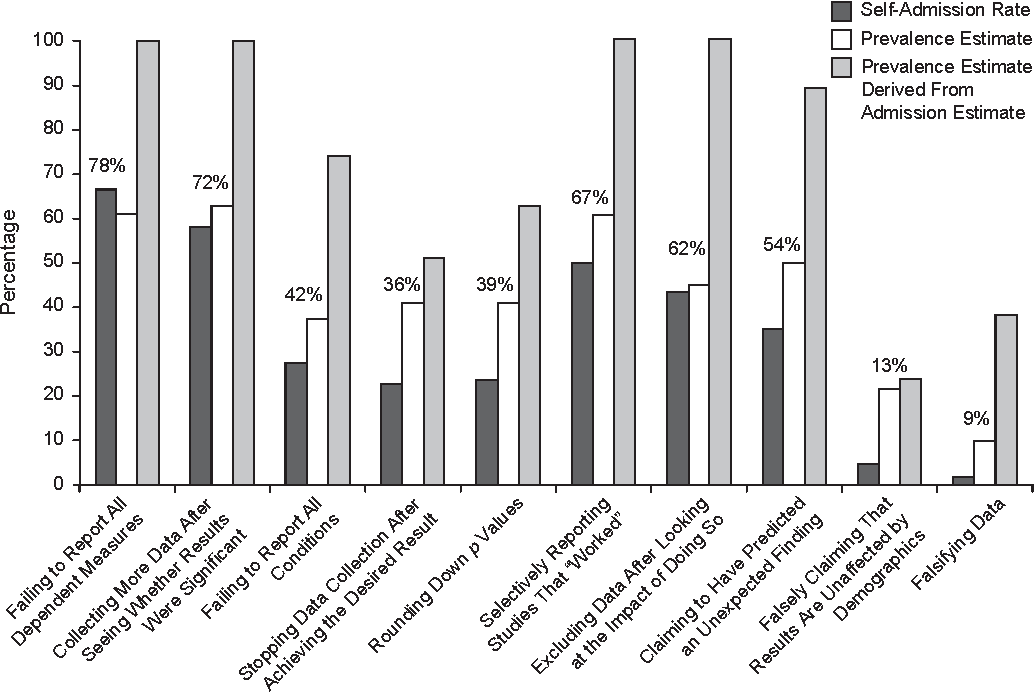
\includegraphics[width=120mm]{./Figures/John2012_Figure1.pdf} \caption{Figure 1 from \textcite{John2012} where the black bars indicate how large proportions of researchers (from a sample of 2,155 academic psychologists in the U.S.) admitted to having engaged in the QRP in question. White bars indicate their estimation of the proportion of other academic psychologists that had engaged in it.} \label{Figure:John2012_Figure1} \end{figure}

No matter the underlying reasons, it can be concluded that if the available research in a certain field were to deviate too much from the actual truth, this would cause major problems when it comes to synthesizing research, such as the studies in this thesis. One should therefore ask to what extent different types of biases and QRP might influence the results of this thesis. Thankfully, there are a number of circumstances that makes it possible to say something about this:

\begin{description} \item [Several successive outcomes.] Within many research fields, the outcome of a study can often only be positive in one specific way while still being consistent with the underlying theory. That is, while it certainly is theoretically possible that cognitive behavioral therapy could affect phobias negatively, such a finding would probably be seen as a failure in finding something real. As such, QRP would probably not tend to lead to this outcome, and studies showing this would presumably not be published.

However, when approaching the research question if there are sex differences for a certain skill or trait, probably all three major conclusions --- that women perform better, that men perform better, and that there are no sex differences --- could potentially be counted as positive findings by most researchers. As such, even if there were no sex differences, and even if QRP were in full effect, one would not expect either sex to ostensibly perform better. Rather, studies showing either that men did better or showing that women did better should be available to about the same extent. Bias inducing mechanisms are therefore less probable when finding overall evidence that a certain sex performs better than what would be the case in many other fields. Or at least, the bias inducing mechanisms would have to be of a more complicated nature, which is less probable.

\item [Studies with other research questions.] As already mentioned in section \ref{Moderators} and presented in the result sections of Study \Romannum{1} and Study \Romannum{2}, not all studies included in the dataset had the explicit goal of investigating sex differences. Rather, in a majority (about 58\%) something else was investigated, suggesting that QRP should not be present for these, at least not in any obvious way. This means that from the start, about half of the dataset probably is not even susceptible to this type of bias, and as shown in the bias analyses for Study \Romannum{1} and Study \Romannum{2} (see the results sections of these studies), whether sex differences were investigated could not be shown to be an influential moderator.

\item [Unpublished findings.] As already mentioned in section \ref{Data_collection}, about 40\% of the data was sent to us from authors after having queried them via email about this possibility. That is, this was previously unpublished results that the authors themselves had not summarized and presented in the article. If data points from studies where other research questions have been investigated are somewhat protected from QRP, data points from studies where the data was not even reported (and presumably, in a lot of cases not even considered) should be even more protected. Obviously, there is an overlap with the previous concept here, meaning that most studies received from authors also fall into the category of studies not investigating sex differences. In addition, both for Study \Romannum{1} and Study \Romannum{2} (as shown in the bias analyses in their respective result sections), whether the data was taken directly from articles or received from authors could not be shown to affect the effect size estimates. \end{description}

Taken together, the reasons listed above should at least alleviate concerns one might have about the underlying data being biased from QRP in some way.

\subsection{Dependent data problem} \label{Dependency} As already mentioned, in section \ref{Hierarchical_structure}, the dataset that we used had a form of hierarchical structure, with dependent data points. However, in a standard meta-analysis, one of the many assumptions concerning the underlying data is that each data point is independent from all the rest. This means that in the total set of effect sizes, $\{e_1, e_2 \dots e_{n}\} \in E$, there should be no clusters of effect sizes, $\{c_1, c_2 \dots c_{n}\} \in C \subseteq E$, where knowing the value of at least one of the cluster effect sizes, $c_x$, will enable you to better predict any of the remaining effect sizes in the cluster, $C \setminus c_{x}$, than any of the effect sizes outside of the cluster, $E \setminus C$. A simple example where this assumption would be violated, even in a dataset where each study only contributes with one data point, is if the same sample of participants has been used in multiple studies. In this case, knowing the effect size from one study where this sample was used would help to better predict other effect sizes where this sample also was used in comparison to effect sizes where it was not used.

This whole dependence issue is a problem because the underlying model in a standard meta-analysis does not take it into consideration. For example, imagine that you had three data points, each derived from different studies, but with equal number of participants, where the standardized differences (that is, Cohen's \emph{d}) are -1, 0, and +1 respectively. Given these numbers, you would have to estimate the true mean difference for the population as 0. But what if you find out that the first and second data points actually come from the same sample? In your original prediction, you gave that sample an unfair weight since it contributes toward two effect sizes and the other only one. To make this point even more clear, imagine that you had 999 effect sizes from one sample and 1 effect size from another. Giving the last effect size the same weighting as any other would render it more or less meaningless in the final estimate even though it would contribute with half of the total amount of participants.

Now, it is important to realize that in practice, clusters like these will always exist in the data, even if they are not as obvious as in the examples above. For example, effect sizes could originate from research performed in the same country, from researchers adhering to the same methodological school, or from experiments conducted in rooms with the same color on the walls. In the end, what constitutes dependency comes down to how much error one is willing to accept. That is, if the color of the room is perceived to only affect the result in a minuscule way, one can ignore this aspect. Most commonly, however, researchers tend to assume that data points are independent from each other as long as each data point is taken from a unique study.

As already mentioned, there is a clear and very influential dependency structure in our dataset where each study can contribute with several different samples, where each sample can contribute with several different encoding sessions, and where each encoding session can contribute with several different measures. Fortunately, there are several ways to deal with this problem \parencite{Hedges2010, Scammacca2014}:

\begin{description} \item [Ignoring it.] One solution to the problem is to simply ignore it and go ahead with the analyses anyway, something that might not be that big of a deal if only a few data points are clustered. In certain situations, this path can even give conservative results that can be used to get a rough overview of the underlying patterns \parencite{Hedges2010}. However, this method is of course not recommended when a high level of accuracy and power is needed.

\item [Data reduction.] The simplest and most straightforward way to actually handle dependent data points (in contrast to just ignoring the problem) is to perform some kind of data reduction/combination procedure to get a dataset without any dependencies that is suitable for the standard meta-analytic method. This could be done either (1) by choosing the most relevant data point from each study or (2) by combining data points within each study in order to end up with non-dependent measures (here, one would sequentially have to combine data points on each hierarchical level, gradually merge combined data points from lower levels until a final measure is achieved). Regarding the first option, this would, in the case of multiple outcome measures, require one to be able to understand which one of these that is the most relevant, and in the case of several samples, one would simply have to keep only one. Discarding data in this way is a problem since this lowers the precision of the final measure. That is, imagine that you measured something 100 times and then were forced to just pick a single data point to keep. Obviously, as long as all type of measurements are relevant, having more of them would enable you to be more sure about the underlying distribution they were sampled from.

Another problem here is that in order to derive a final variance measure for the combination procedure, one also has to specify an assumed correlation between the data points. If this correlation is set to 1, it does not matter how many times you measure something; the final measure will not be more precise than if you only measured it once. On the other hand, if this correlation is set to 0, gathering more data points will always increase the precision of the final measure. Correlations between data points can often be hard to know (or even hard to just estimate), and they might very well differ between different tasks, samples, and studies. This means that when not having access to the original raw data of each study (which one very seldom do), the best one can do is to err on the side of caution and choose a correlation that almost surely is too conservative.

Finally, when using one of these methods, in order to carry out moderator analyses with not more than two levels, one would first have to derive two separate measures for each level within each cluster (that still would be dependent in relation to each other) and then subtract one from the other. This would result in a difference score for each cluster, that then could be used in a standard moderator meta-analysis. However, performing moderator analyses with moderators with even more levels is not possible when using this method.

\item [Specifying the covariance structure.] If the covariance structure between dependent data points, discussed above, is known or if a reasonable estimation of it can be made, it is possible to to use it within a multivariate model directly (see, for example, \citeauthor{Hripsime1996}, \citeyear{Hripsime1996}). Here, if this covariance structure is accurate enough, this method is the also the most accurate one to use. However, as already touched on above, unless one has access to the raw data, making the necessary estimations are both very hard and time consuming. It is, however, also possible to conduct sensitivity analyses, using different covariance structures to see how the result may vary when utilizing different estimates.

\item [Leaving out the covariance structure.] As discussed several times above, finding out or estimating the covariance structure between dependent data points can be an extremely time-consuming task, and in many cases it can be almost impossible to derive good enough estimates. In these cases, there are two methods that can be used: \emph{Robust variance estimation} \parencite{Hedges2010} and \emph{n-level meta-analysis}\footnote{The term \emph{n} here stands for the number of levels that the model has, where the most simple meta-analytical model has two: One modeling the between-studies variance and one modeling the within-studies variance (or error variance). As such, when having clusters of studies from, for example, different research labs, this would warrant a three-level meta-analysis (with research labs being the third one).} \parencite{Konstantopoulos2011}. Both these models can, albeit differently, handle not having access to what degree dependent data points covary, and also handle hierarchically clustered data. \end{description}

\textcite[p. 81]{Hoare1980} concluded that ``there are two ways of constructing a software design: One way is to make it so simple that there are \emph{obviously} no deficiencies, and the other way is to make it so complicated that there are no \emph{obvious} deficiencies.'' The same thing goes for statistics where you often have to choose between methods that are simple/easy to understand and methods that are more complicated/hard to understand. As such, going with the simple alternative might be less accurate but more transparent and easier to assess by a reader. On the other hand, going with the more complicated option might be more accurate (if one applies it correctly, which might be harder to do) but less transparent and harder to assess for the recipient.

For the data that constituted the basis of this thesis, going with any of the first two methods (ignoring the problem or perform some kind of data reduction) would, to paraphrase Hoare, be \emph{obviously} wrong; using the data reduction method would still mean that data points were dependent for moderator analyses with more than two levels.\footnote{Even if, for Study I, we used the data reduction method (more specifically, the combination procedure) to compute descriptive effect sizes for each study in Table S2 (not included in this thesis; see \citeauthor{Asperholm2019}, \citeyear{Asperholm2019}) and to generate the data points that made up the basis for the funnel plots for each material category subset in Figures S2 to S10. The exact method that was used for this combination procedure is described in the caption of Figure S1 (which \emph{is} included in this thesis).} On the other hand, the third alternative (specifying the covariance structures) would require information that simply was not available, neither could it be estimated in a reasonable way. Remember that the large heterogeneity of the different types of tasks would make it necessary to come up with about as many dependency structure estimations as there are unique tasks and ways of measuring the outcomes of those very tasks.

Thus, we are left with the fourth, fairly complicated alternative (leaving out the covariance structure), which might be quite hard for the general reader to grasp. Here, I opted for n-level meta-analyses, somewhat because of the incidental circumstances that a reviewer of Study \Romannum{1} suggested it and that I already had some experience using the \emph{Metafor} package \parencite{Viechtbauer2010} for \emph{R}, which has the capacity to carry out these type of analyses.

\subsection{Ethical considerations}

Before ending this thesis, I should spend some time reflecting on possible ethical problems with the studies that we conducted when it comes to \emph{how} it was being done (while section \ref{Why_study_sex?} more deals with aspects of \emph{why} it should be done). In Study \Romannum{1}, \Romannum{2}, and \Romannum{3}, all analyses are based on the same dataset, a dataset that is made up of aggregated numbers from already published articles and open databases. In some cases, we received data from authors, but the form of this data did not differ from what already was published (that is, aggregated numbers describing groups). Further, the open databases we used were, as the name suggests, more or less open already, available for just about anyone who can manage the hassle of going through a short registration process. As such, the data and results are not any more traceable back to the original participants than they were in their original form in the different articles and open databases (if anything, it is harder). No ethical concerns with regard to the anonymity of participants should therefore be present for these studies.

However, while the tasks that were investigated in our dataset can be said to probably not cause any harm to the participants, it is of course impossible to guarantee this or that other unethical research practices were not utilized. Scientific journals have certain standards that the authors need to follow in order to get published, but these standards can still be circumvented since no rigorous control normally is being performed. As such, it \emph{could} be the case that we, to a certain extent, base our findings on unethical studies. However, we have no indications that this would be the case, and even if it unbeknownst to us were the case, it is debatable to what extent this would further hurt the participants.

\subsection{Concluding thoughts}

As with all scientific endeavors, pretty much nothing is ever the final nail in the coffin for anything. Within the span of a Ph.D., you can often, at best, hope to nudge the knowledge within a field in one way or another. For this thesis, I hope (and feel) that I have contributed to this nudging process. The results presented might not have been extremely novel, but they have nevertheless hopefully helped us to get a more firm grip about the state of things when it comes to sex differences in episodic memory.
